% Importamos el preámbulo con la configuración del documento
% Definición de la clase del documento
\documentclass[a4paper, 11pt]{book} % A4 paper and 11pt font size

% Entrada y salida de texto
\usepackage[T1]{fontenc}
\usepackage[utf8]{inputenc}
\usepackage[sfdefault]{roboto} % Option 'sfdefault' only if the base font of the document is to be sans serif

% Idioma
\usepackage[spanish, es-tabla]{babel} % Selecciona el español y el uso de la palabra "tabla" en lugar de "cuadro"

% Información reutilizable
\newcommand{\asunto}{Trabajo de Fin de Grado}
\newcommand{\titulo}{Juego de tablero aumentado utilizando ARCore}
\newcommand{\tituloEng}{Augmented board game using ARCore}
\newcommand{\subtitulo}{Desarrollo de un juego de mesa aumentado mediante uso de tecnologías de realidad aumentada}
\newcommand{\subtituloEng}{Development of augmented board game using augmented reality technologies}
\newcommand{\grado}{Grado en Ingeniería Informática}
\newcommand{\autor}{Miguel Ángel Torres López}
\newcommand{\email}{matl1995@correo.ugr.es}
\newcommand{\tutor}{Francisco Luis Gutiérrez Vela}
\newcommand{\escuela}{Escuela Técnica Superior de Ingenierías Informática y de Telecomunicación}
\newcommand{\departamento}{Departamento de Lenguajes y Sistemas Informáticos}
\newcommand{\universidad}{Universidad de Granada}
\newcommand{\ciudad}{Granada}
\providecommand{\keywords}{ARCore, Unity, Android, juegos de mesa}
\providecommand{\keywordsEng}{ARCore, Unity, Android, board games}

% Otros paquetes importantes para el proyecto
\usepackage[hyphens]{url}
\usepackage{eurosym}
\usepackage{graphicx}
\usepackage{colortbl}
\usepackage{fancyhdr}
\usepackage{pdfpages}
\usepackage{longtable}
\usepackage[hidelinks]{hyperref}
\usepackage{placeins}
\usepackage{verbatim}

\setcounter{tocdepth}{4}
\setcounter{secnumdepth}{4}

% Añade aquí las carpetas de imágenes para que el compilador las pueda analizar
\graphicspath{{../images/}{../screenshots/}{../images/applications/}{../images/integration/}{../images/techniques/}{../images/mockups/}{../images/headmounted/}{../images/tangibleinterfaces/}{../images/estudiomercado1/}{../images/estudiomercado2/}{../images/metodologias/}{../images/desarrollo/}{../images/entrega2/}}

% Información del archivo
\hypersetup{
  pdfauthor = {\autor\ (\email)},
  pdftitle = {\titulo: \subtitulo},
  pdfsubject = {\asunto},
  pdfkeywords = {\keywords},
  pdfcreator = {LaTeX, con la distribución TeX Live},
  pdfproducer = {pdflatex}
}

% Modificación para que las páginas en blanco no tengan cabecera
\makeatletter
\def\clearpage{
  \ifvmode
    \ifnum \@dbltopnum = \m@ne
      \ifdim \pagetotal < \topskip
        \hbox{}
      \fi
    \fi
  \fi
  \newpage
  \thispagestyle{empty}
  \write\m@ne{}
  \vbox{}
  \penalty -\@Mi
}
\makeatother

% Definición del estilo de las cabeceras
\pagestyle{fancy}
\fancyhf{}
\fancyhead[LO]{\leftmark}
\fancyhead[RE]{\rightmark}
\fancyhead[RO,LE]{\textbf{\thepage}}
\setlength{\headheight}{1.5\headheight}

% Definición de colores
\definecolor{Gray}{gray}{0.9}

% Redefinición de comandos
\renewcommand{\chaptermark}[1]{\markboth{\textbf{#1}}{}}
\renewcommand{\sectionmark}[1]{\markright{\textbf{\thesection. #1}}{}}
% \renewcommand{\lstlistingname}{Fragmento de código}
% \renewcommand{\lstlistlistingname}{Índice de fragmentos de código}

% Creación de comandos
% \newcommand{\HRule}{\rule{\linewidth}{0.5mm}}
% \newcommand{\bigrule}{\titlerule[0.5mm]}

% Ajuste para minimizar el fragmentado de listados
% \lstnewenvironment{listing}[1][]
%   {\lstset{#1}\pagebreak[0]}{\pagebreak[0]}


\begin{document}

% Portada del documento
\begin{titlepage}

\newlength{\centeroffset}
\setlength{\centeroffset}{-0.5\oddsidemargin}
\addtolength{\centeroffset}{0.5\evensidemargin}

\noindent\hspace*{\centeroffset}

\begin{minipage}{\textwidth}

\centering


\includegraphics[width=0.9\textwidth]{logo_ugr}\\[1.4cm]

\textsc{\Large\asunto\\[0.2cm]}
\textsc{\grado}\\[1cm]

{\Huge\bfseries\titulo\\}
\noindent\rule[-1ex]{\textwidth}{3pt}\\[3.5ex]
{\large\bfseries\subtitulo}

\end{minipage}

\vspace{1.5cm}
\noindent\hspace*{\centeroffset}

\begin{minipage}{\textwidth}

\centering

\textbf{Autor}\\{\autor}\\[2.5ex]
\textbf{Tutor}\\{\tutor}\\[1.5cm]


\includegraphics[width=0.3\textwidth]{logo_etsiit}\\[0.1cm]

\textsc{\escuela}\\
\textsc{---}\\
\ciudad, \today\\

\end{minipage}

\end{titlepage}


% Prefacio del documento
\cleardoublepage
\thispagestyle{empty}

\begin{center}
{\LARGE\bfseries\titulo: \subtitulo}\\
\end{center}
\begin{center}
\autor
\end{center}

\bigskip
\noindent{\textbf{Palabras clave}: \textit{\keywords}\\

\section*{Resumen}
Este documento expone mi trabajo de fin de grado, y los contenidos asociados al mismo.\\

Este proyecto se va a centrar en la planificación y desarrollo de un juego de mesa, que mediante las tecnologías de realidad aumentada, mas concretamente ARCore, aportará un nuevo enfoque sobre los juegos de esta temática, aprovechando las singulares características que la realidad aumentada ofrece.\\

El objetivo principal del juego es explorar que ventajas puede aportar la realidad aumentada a los juegos en dispositivos móviles, y mas específicamente a los juegos de mesa en dispositivos móviles.\\

El proyecto explorará también la integración de diferentes formas de interacción en juegos, permitiendo funcionalidades que se tendrán que llevar a cabo mediante interacción con elementos físicos, y otras funcionalidades que se desarrollarán con interacción únicamente con el dispositivo móvil.\\

\cleardoublepage
\thispagestyle{empty}

\begin{center}
{\LARGE\bfseries\tituloEng: \subtituloEng}\\
\end{center}
\begin{center}
\autor
\end{center}

\bigskip
\noindent{\textbf{Keywords}: \textit{\keywordsEng}\\

\section*{Abstract}
This document shows my end-of-degree project and the contents associated with it.\\

This project will focus on the planning and development of a board game, that using the augmented reality technologies available, specifically using ARCore, will bring a new approach to the games of this theme, taking advantage of the singular characteristics that augmented reality offers.\\

The main objective of the game is to explore the advantages that augmented reality can bring to mobile devices games, and more specifically to board games in mobile devices.\\

The project will also explore the integration of different ways of interaction in games, allowing functionalities that will have to be done by interacting with physical elements, and other functionalities that will have to be done interacting only with the mobile device.\\

\chapter*{}
\thispagestyle{empty}

\noindent\rule[-1ex]{\textwidth}{2pt}\\[4.5ex]

Yo, \textbf{\autor}, alumno de la titulación \textbf{\grado} de la \textbf{\escuela} de la \textbf{\universidad}, con DNI 71358141C, autorizo la ubicación de la siguiente copia de mi Trabajo de Fin de Grado en la biblioteca del centro para que pueda ser consultada por las personas que lo deseen.\\

Así mismo, el código fuente del proyecto y esta documentación pueden consultarse en la dirección \url{https://github.com/matl1995/TFG} para que aquellos que lo deseen puedan probar el proyecto.

\vspace{5cm}

\noindent \textbf{Fdo: \autor}

\vspace{2cm}

\begin{flushright}
\ciudad, a \today
\end{flushright}

\chapter*{}
\thispagestyle{empty}

\noindent\rule[-1ex]{\textwidth}{2pt}\\[4.5ex]

D. \textbf{\tutor}, profesor del \textbf{\departamento} de la \textbf{\universidad}.

\vspace{0.5cm}

\textbf{Informa:}

\vspace{0.5cm}

Que el presente trabajo, titulado \textit{\textbf{\titulo: \subtitulo}}, ha sido realizado bajo su supervisión por \textbf{\autor}, y autoriza la defensa de dicho trabajo ante el tribunal que corresponda.

\vspace{0.5cm}

Y para que conste, expide y firma el presente informe en \ciudad, a \today.

\vspace{1cm}

\textbf{El tutor:}

\vspace{5cm}

% \begin{figure}[H]
% \includegraphics[width=0.3\textwidth]{firma_tutor}
% \end{figure}

\noindent\textbf{\tutor}

\chapter*{Agradecimientos}
\thispagestyle{empty}

\vspace{1cm}

A mi tutor del TFG por toda la ayuda y apoyo durante el proyecto.\\

A mi familia por estar ahi siempre que lo he necesitado.\\

A mis amigos y amigas por todas las veces que me han ayudado y apoyado durante todas las etapas de mi vida.\\

A mis profesores por su incansable esfuerzo durante estos años de carrera para que aprendamos lo máximo posible y de la mejor manera.\\


\frontmatter
\begingroup
\let\cleardoublepage\clearpage
  \tableofcontents
  % \listoffigures
  % \listoftables
  % \lstlistoflistings
\endgroup

\newpage
\thispagestyle{empty}

% Capítulos del documento
\mainmatter
\chapter{Introducción y objetivo}
\label{ch:introduccion}

\section{Introducción}
La realidad aumentada es una tecnología que está en pleno auge, no paramos de ver noticias que nos muestran todo lo que esta permite, las diferentes utilizades que tiene y como va a mejorarnos la vida. No obstante esto no era así hace un año, como se puede observar en el grafico del "Hype Cycle" de Gartner sobre tecnologías emergentes en 2017, Figura \ref{figura-gartner}, la realidad aumentada se situaba en el tramo de desilusión, lo que significa que despues de estar en lo alto de la gráfica años anteriores, cuando se hablaba mucho de la tecnología y todo lo que ofrecía, en julio de 2017 se encontraba en lo mas bajo, apenas se hablaba de dicha tecnología, lo que significa que aun hay mucho por hacer, y queda mucho por trabajar sobre esta tecnología.\\

\begin{figure}[h]
  \centering
  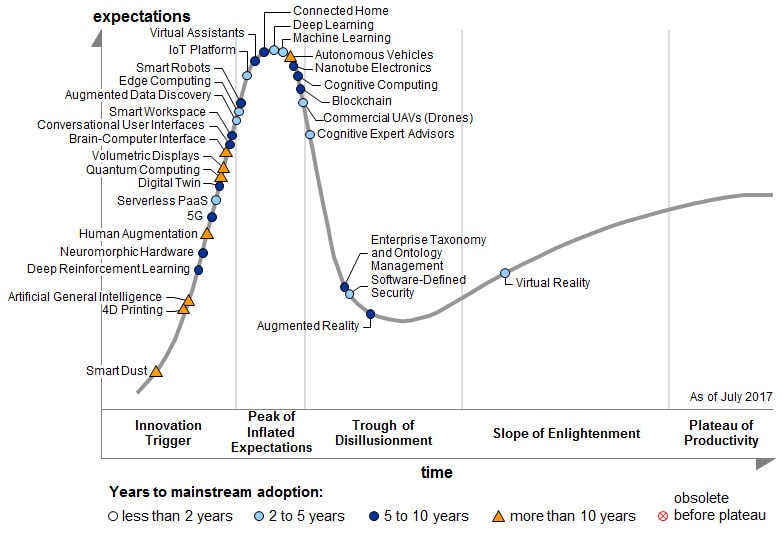
\includegraphics[scale=0.5]{gartner-hype-cycle}
  \caption{Imagen que muestra el "Hype cycle" de Gartner para tecnologías emergentes en 2017.\protect\footnotemark}
  \label{figura-gartner}
\end{figure}

\footnotetext{ \url{https://www.gartner.com/newsroom/id/3784363}, Gartner (July 2017)}

Sin embargo, desde que Apple y Google lanzaran sus respectivas librerías hace apenas un año, la realidad aumentada ha mejorado su situación notablemente, distanciándose de la realidad aumentada vista hasta el momento, estas nuevas librerias permiten, con los componentes de un dispositivo móvil de masas sea posible reconocer y entender el mundo que le rodea, así como su posición en el mundo. Esto supone una diferenciación en las tecnologías hasta entonces presentes, que o bien necesitaban de mucho hardware para ser capaces de conseguir esto, o en dispositivos móviles de masas, tenían capacidades reducidas.\\

Actualmente la realidad aumentada abre un mundo de grandes posibilidades que pueden revolucionar muchos ámbitos, entre ellos el de los juegos, un juego ya no tiene que quedarse dentro de una pantalla o un mundo virtual, ahora puede dar el salto el mundo real, esto aporta un grado de realismo y espectacularidad que puede suponer una reinvención de los juegos como ahora los conocemos.\\

Por otro lado, la mayoría de la población dispone de un dispositivo móvil, como podemos ver en la Figura \ref{figura-ine}, en el año 2017, un 97.4\% de los hogares españoles contaba con al menos un dispositivo móvil \cite{ine}, esto implica que casi la totalidad de los españoles tiene acceso a dispositivos móviles, y por tanto, a las aplicaciones que utilizan realidad aumentada.

\begin{figure}[h]
  \centering
  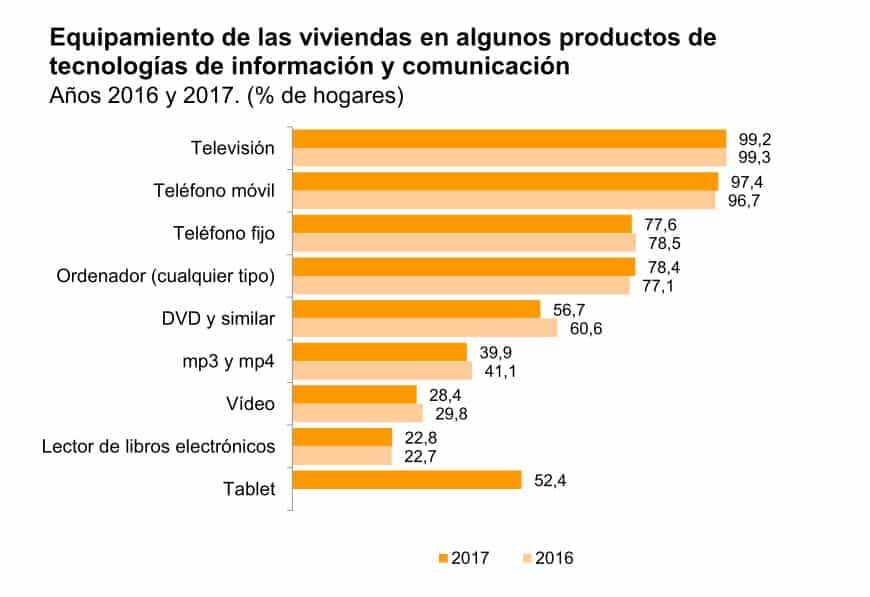
\includegraphics[scale=0.4]{ine2017}
  \caption{Imagen que muestra los porcentajes de hogares que cuentan con cada dispositivo tecnológico.\protect\footnotemark}
  \label{figura-ine}
\end{figure}

\footnotetext{{\em Encuesta sobre Equipamiento y Uso de Tecnologías de la Información y Comunicación en los Hogares.} INE, B. (2017).}

\newpage

\section{Motivación}
Personalmente el estar una gran parte del tiempo de cada dia utilizando mi teléfono móvil y jugando con el me despertó la curiosidad acerca de como se desarrollan los videojuegos, y que es lo que hay detras del producto que al final el usuario descarga de una tienda de aplicaciones.\\

Por otro lado, mi interés por el desarrollo del software me lleva a querer conocer y explorar este mundo, la experiencia de planificar y desarrollar un proyecto software al completo por mi mismo.\\

Las nuevas tecnologías siempre me han llamado la atención y me gusta estar informado sobre ellas, y viendo la revolución de la realidad aumentada me pareció un mundo apasionante por las capacidades ofrece, el poder fusionar el mundo virtual y real, y llevar a cabo aplicaciones y juegos con ella, me pareció algo fascinante y que sin duda me gustaría explorar.\\

La amplia disponibilidad de dispositivos móviles entre la población, y el alto nivel de uso diario que hacen los usuarios de estos, hace del desarrollo para estos dispositivos algo atractivo, ya que es probablemente la mayor plataforma para desarrolladores de software actualmente.\\

Esto en conjunto con el crecimiento de la realidad aumentada, hace que un juego para dispositivos móviles que hace uso de esta tecnología, sea una opción muy interesante para un proyecto, que permite adquirir conocimientos en el desarrollo de videojuegos, en el desarrollo de aplicaciones móviles, y exploarar la realidad aumentada y lo que puede aportar a las aplicaciones de dispositivos móviles actuales.

\section{Estructura del documento}
Este documento se divide en 4 capítulos, a continuación se detalla el contenido de cada uno de los capítulos del documento:
\begin{itemize}
  \item \textbf{Capítulo 1, Introducción y objetivo:} En este capítulo se hace una pequeña introducción al proyecto, explicando la motivación por la que surgió el proyecto, la estructura del documento, y también se exponen los objetivos que han sido establecidos para este proyecto.
  \item \textbf{Capítulo 2, Estado del arte:} En este capítulo se hará una exposición de cual es el estado actual de la realidad aumentada, diferencias con tecnologías similares, que aplicaciones tiene, etc.
  \item \textbf{Capítulo 3, Análisis inicial del problema:} En este capítulo se llevará acabo un analisis de cual es el problema y como este puede ser resuelto.
  \item \textbf{Capítulo 4, Metodologías a usar en el proyecto:} En este capítulo se recogen las diferentes metodologías utilizadas para el desarrollo del proyecto, y se explica como serán utilizadas en el proyecto.
  \item \textbf{Capítulo 5, Plan de entregas:} En este capítulo se detalla el plan de entregas llevado a cabo, y las historias de usuario realizadas para definir los requisitos que tendrá el sistema.
  \item \textbf{Capítulo 6, Desarrollo. Entregas e iteraciones:} En esta capitulo se recogerá el trabajo realizado durante las diferentes iteraciones, así como el resultado de las distintas entregas.
  \item \textbf{Capítulo 7, Conclusiones y Trabajos Futuros:} En este capítulo se recoge el resultado del proyecto, las conclusiones obtenidas del desarrollo de éste y los trabajos futuros a realizar en el proyecto.
\end{itemize}

\section{Objetivo}
El objetivo principal de este proyecto es explorar que ventajas puede aportar la realidad aumentada, mas concretamente el SDK ARCore, a los juegos en dispositivos móviles, y mas específicamente a los juegos de mesa en dispositivos móviles. Por tanto, mediante este proyecto se adquirirá experiencia en el desarrollo con tecnologías de realidad aumentada.\\

Objetivos secundarios:
\begin{itemize}
  \item Investigar una implementación para juegos de mesa virtuales que aporte un enfoque diferente al habitual.
  \item Adquirir conocimientos sobre la planificación y desarrollo de proyectos de software, mas concretamente de videojuegos.
  \item Adquirir conocimientos sobre la realidad aumentada, como ésta funciona y cuales son las mejores SDK para desarrollar utilizando dicha tecnología.
\end{itemize}

\chapter{Estado del arte}
\label{ch:estado}

\section{Realidad aumentada}
Una de las primeras definiciones de realidad aumentada fue dada por Ronald Azuma en 1997 \cite{azuma}, y dice que la Realidad Aumentada es cualquier sistema que combine elementos reales y virtuales, que sea interactivo en tiempo real y que sea registrado en tres dimensiones. Por tanto, la realidad aumentada es una tecnología que permite añadir información virtual al mundo real a través de un dispositivo, es decir, permite mostrar el mundo real con objetos virtuales en éste, por lo que no pretende crear un mundo virtual, sino complementar al mundo real con más información.

\section{Diferencias entre realidad aumentada, realidad virtual y realidad mixta}
Las diferencias entre estas tres tecnologías son las siguientes \cite{intel}:

\begin{itemize}
  \item \textbf{Realidad virtual}: Es una tecnología completamente inmersiva que consiste en convencer a tus sentidos de que estas en otro mundo que no es el real, es un mundo virtual. Usando un dispositivo que se coloca en la cabeza, la realidad virtual permite disfrutar de un mundo de imágenes y sonidos generado por ordenador en el que se puede manipular objetos, y moverse por dicho mundo usando controladores hápticos conectados a un ordenador o a una consola.

  \item \textbf{Realidad aumentada}: Es una tecnología que superpone información digital sobre elementos del mundo real. El elemento central es el mundo real, pero lo mejora con otros detalles digitales, complementando así la realidad.

  \item \textbf{Realidad mixta}: Es una tecnología que hace converger el mundo real y elementos digitales. En esta puedes interactuar y manipular tanto elementos físicos como virtuales. La realidad mixta te permite sumergirte en el mundo que te rodea incluso cuando tú interactúas con el entorno virtual usando tus propias manos. Esta tecnología te permite tener un pie en el mundo real y el otro en un lugar imaginario.
\end{itemize}

\section{Aplicaciones de la realidad aumentada}
Para comprender mejor las posibilidades que la realidad aumentada ofrece, a continuación se muestrán diferentes aplicaciones que esta puede tener y ejemplos de dichas aplicaciones en funcionamiento que son bastante interesantes:

\begin{itemize}
  \item \textbf{Medicina}: La realidad aumentada puede aportar grandes avances a la medicina, ya que permite la visualización en 3D de objetos que bien pueden ser órganos o partes del cuerpo en el mundo real, por lo que puede facilitar a los doctores muchas tareas que requieran el estudio de modelos 3D. Por ejemplo, los doctores pueden utilizar la realidad aumentada con el objetivo de prepararse para una operación como se puede observar en la Figura \ref{figura-medicina}, o simplemente para tareas de visualización médica, de igual manera que actualmente se utilizan los TAC o las resonancias magnéticas, pero los datos obtenidos con dichos escáneres se convertirían en modelos 3D que son mucho más sencillos de explorar que un conjunto de imágenes 2D. También se podría utilizar la realidad aumentada con el objetivo de entrenamiento para cirujanos que se están formando, mostrándoles instrucciones sobre un modelo 3D de cómo se debería realizar una determinada operación, ayudando así a que no necesiten consultar un manual y quitar la vista del “paciente” si no que todo sería sobre dicho “paciente” que realmente es un modelo 3D \cite{azuma}.

  \begin{figure}[h]
    \centering
    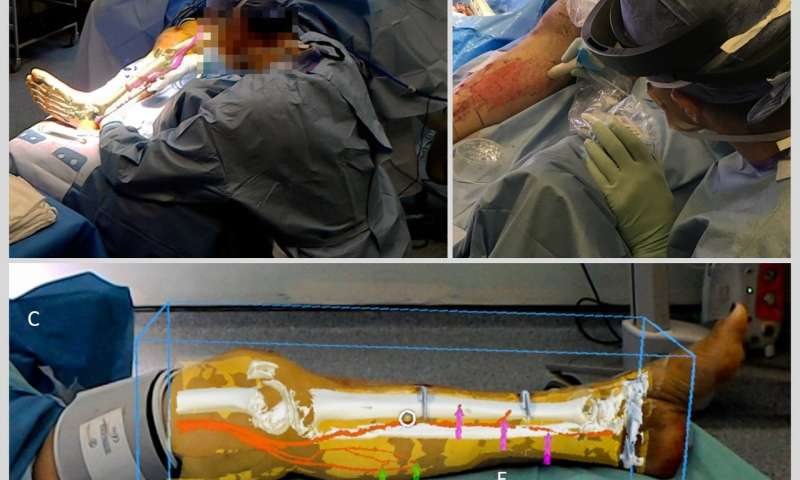
\includegraphics[scale=0.5]{medicine}
    \caption{Profesionales médicos utilziando realidad aumentada como ayuda para una operación.\protect\footnotemark}
    \label{figura-medicina}
  \end{figure}

  \footnotetext{ Philip Pratt, et al. Eur Radiol Exp, 2018}

  \newpage

  \item \textbf{Educación}: La realidad aumentada tiene mucho que aportar a la educación, ya que permite una forma interactiva de aprender que los libros no permiten. Por ejemplo, que mejor manera de aprender el sistema respiratorio que con uno a tamaño real en 3D que tu puedes explorar. Y la realidad aumentada no implica que los libros no sirvan y vayan a desaparecer, si no que puede suponer un complemento para dichos libros como se puede observar en la Figura \ref{figura-educacion}, cambiando la forma en la que nos relacionamos con ellos, por ejemplo, con imágenes en los libros que al escanearlas muestren elementos 3D que nos permitan comprender mejor el contenido que se está exponiendo en dicho libro \cite{reinoso}.

  \begin{figure}[h]
    \centering
    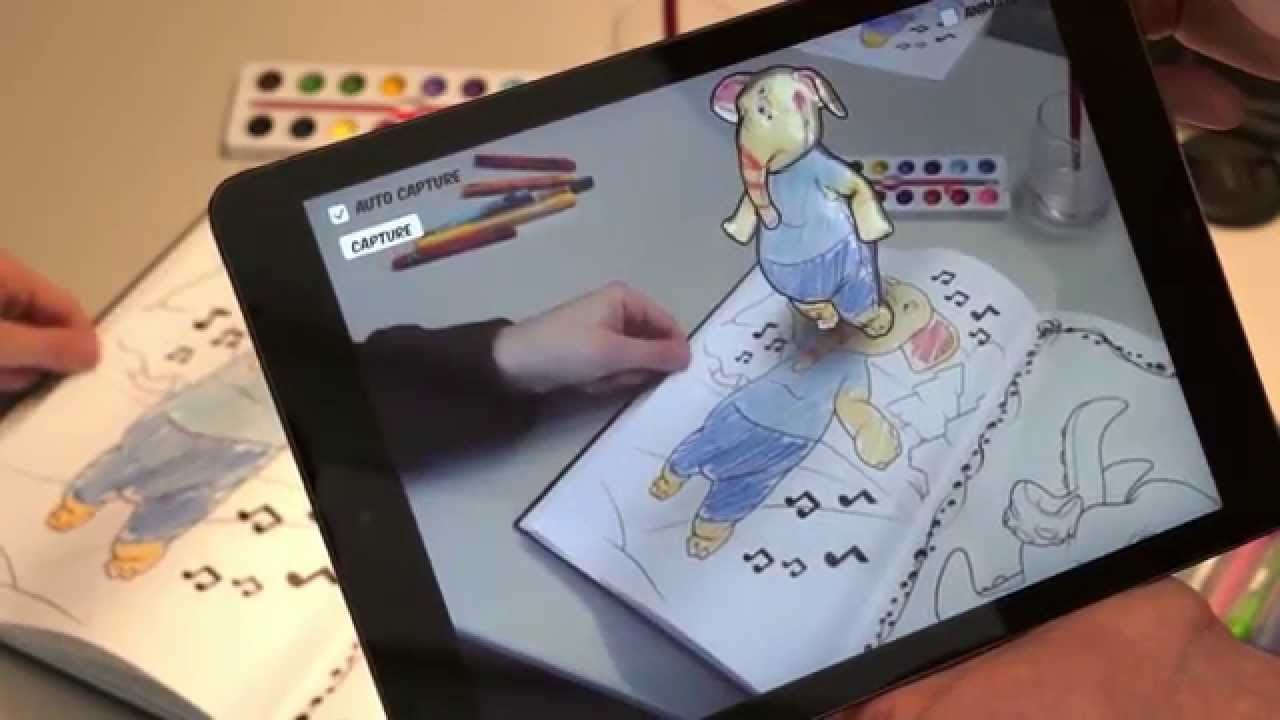
\includegraphics[scale=0.2]{education}
    \caption{Libro que utiliza la realidad aumentada para mostrar el dibujo en 3D.\protect\footnotemark}
    \label{figura-educacion}
  \end{figure}

  \footnotetext{ \url{https://www.youtube.com/watch?v=IeHKVC0XLe4}, Alibabach}

  \begin{figure}[h]
    \centering
    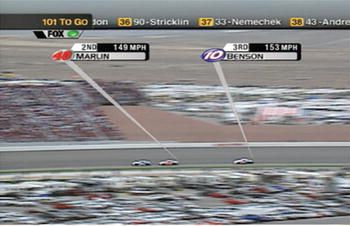
\includegraphics[scale=0.7]{entertainment1}
    \caption{Imagen que muestra la utilización de realidad aumentada en la retransmisión de deportes. \cite{van-krevelen}}
    \label{figura-entretenimiento1}
  \end{figure}

  \item \textbf{Entretenimiento}: La realidad aumentada se puede aplicar en el entretenimiento relacionada a juegos, por ejemplo, mostrando los tableros de juego en una superficie plana en lugar de en la pantalla en 2D, como se puede ver en la Figura \ref{figura-entretenimiento}, pero también se puede aplicar la realidad aumentada en otras formas de entretenimiento diferentes, por ejemplo, en los deportes que se retransmiten, mostrando información relevante para los usuarios sobre dicho deporte, por ejemplo, en las carreras de coches, ya que puede estar grabado desde cierta distancia mostrar sobre cada coche información de quien es, su puesto y la velocidad que lleva como se puede ver en la Figura \ref{figura-entretenimiento1} \cite{van-krevelen}.

  \begin{figure}[h]
    \centering
    
\includegraphics[scale=0.1]{entertainment}
    \caption{Imagen que muestra la utilización de realidad aumentada en un juego.\protect\footnotemark}
    \label{figura-entretenimiento}
  \end{figure}

  \footnotetext{ \url{https://itunes.apple.com/us/app/stack-ar/id1269638287?mt=8}, Ketchapp}

  \item \textbf{Turismo}: La realidad aumentada puede dar una vuelta al turismo, teniendo un guia turistico en tu propio dispositivo móvil, por ejemplo, mediante el uso de realidad aumentada que utiliza la geolocalización, puede indicar los monumentos relevantes de la ciudad, la distancia a ellos y donde están a través de la cámara de un dispositivo móvil. También puede mejorar las experiencias turísticas actuales de una forma mucho más visual, cuando se esté en un sitio histórico te puede contar la historia de una forma más entretenida y visual, mostrando elementos 3D en el lugar, recreando lo que sucedió, como se puede observar en la Figura \ref{figura-turismo} \cite{reinoso}.

  \begin{figure}[h]
    \centering
    
\includegraphics[scale=0.15]{turism}
    \caption{Imagen que muestra un hecho historico visualizandose con realidad aumentada. \cite{layar}}
    \label{figura-turismo}
  \end{figure}

  \newpage

  \item \textbf{Comercio}: La realidad aumentada puede revolucionar el sector de las ventas por internet, la mayor desventaja actual que tiene comprar por internet es que el usuario se tiene que conformar con imágenes 2D del producto, la realidad aumentada permite romper esa barrera, y mostrar al usuario el producto en 3D, en tamaño real en su propia casa, por ejemplo, esto es muy útil con muebles ya que necesitas las medidas del hueco que tienes y del mueble para saber si encajará en el hueco o simplemente si queda bonito en la habitación, con la realidad aumentada ambos problemas están solucionados, puedes ver el mueble en el hueco que quieres en tamaño real, lo que te permite saber si cabe y si queda bien. Un ejemplo de este tipo de aplicación se puede observar en la Figura \ref{figura-comercio}.

  \begin{figure}
    \centering
    
\includegraphics[scale=0.3]{commerce}
    \caption{Imagen que muestra la utilización de realidad aumentada en un juego.\protect\footnotemark}
    \label{figura-comercio}
  \end{figure}

  \footnotetext{ \url{https://itunes.apple.com/es/app/ikea-place/id1279244498?mt=8}, Ikea}

\end{itemize}

\newpage

\section{Formas de integrar la información digital con el mundo real}
A la hora de trabajar con realidad aumentada, es necesario que la información que se situe en el mundo real vaya vinculada a un elemento, a continuación se listan los diferentes elementos a los que se puede vincular la información en una aplicación de realidad aumentada \cite{prendes-espinosa}:

\begin{itemize}
  \item \textbf{Vincular la información a un marcador}: Un marcador es una imagen en blanco y negro que contiene un patrón, como puede ser un código QR, un ejemplo de marcador se puede ver en la Figura \ref{figura-marcador}. Este tipo de tecnologóia almacena en memoria marcadores, y cuando se escanea dicho marcador se puede mostrar una información asociada a este con respecto a la posición de dicho marcador, como se puede ver en la Figura \ref{figura-marcador-aumentado}.

  \begin{figure}
    \centering
    
\includegraphics[scale=0.3]{marker}
    \caption{Imagen que muestra un ejemplo de marcador.}
    \label{figura-marcador}
  \end{figure}

  \begin{figure}[h]
    \centering
    
\includegraphics[scale=0.5]{marker-augmented}
    \caption{Imagen que muestra un marcador con un modelo 3D asociado a este.\protect\footnotemark}
    \label{figura-marcador-aumentado}
  \end{figure}

  \footnotetext{ \url{http://www.himix.lt/augmented-reality/augmented-reality-using-armedia/}, Himix}

  \newpage

  \item \textbf{Vincular la información a una imagen fija o móvil}: Lo que hace es almacenar en memoria imágenes, y cuando dichas imágenes se escanean se puede mostrar una información asociada a dicha imagen con respecto a la posición de la imagen, cabe la posibilidad de que cuando dicha imagen esté en movimiento se pierda la información asociada a esta y se muestre cuando vuelva a estar fija, o por el contrario que dicha información asociada se desplace junto con la imagen. Podemos observar un ejemplo en la Figura \ref{figura-image}.

  \begin{figure}[h]
    \centering
    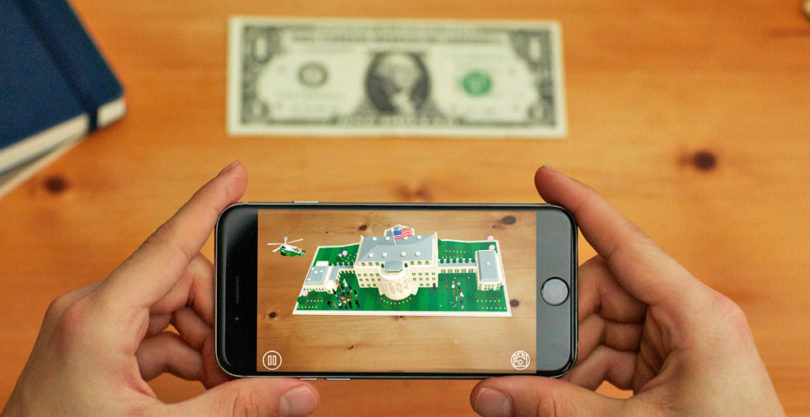
\includegraphics[scale=0.3]{image}
    \caption{Imagen que muestra una imagen con un modelo 3D asociado a esta.\protect\footnotemark}
    \label{figura-image}
  \end{figure}

  \footnotetext{ \url{https://vrscout.com/news/augmented-reality-app-1-dollar-bill-tour-white-house/}, Kyle Melnick}

  \newpage

  \item \textbf{Vincular la información a un objeto 3D}: Este proceso funciona de manera que en memoria se almacena un modelo 3D, posteriormente cuando se escanea el entorno se escanean los objetos en este, y se contrasta la información obtenida del escaneo con el modelo 3D que esta en memoria (esto es posible con dispositivos como Kinect que se muestra en la Figura \ref{figura-kinect}), si el modelo 3D en memoria coincide con el objeto 3D que se encuentra en la escena se puede asociar una información virtual a dicho objeto.

  \begin{figure}[h]
    \centering
    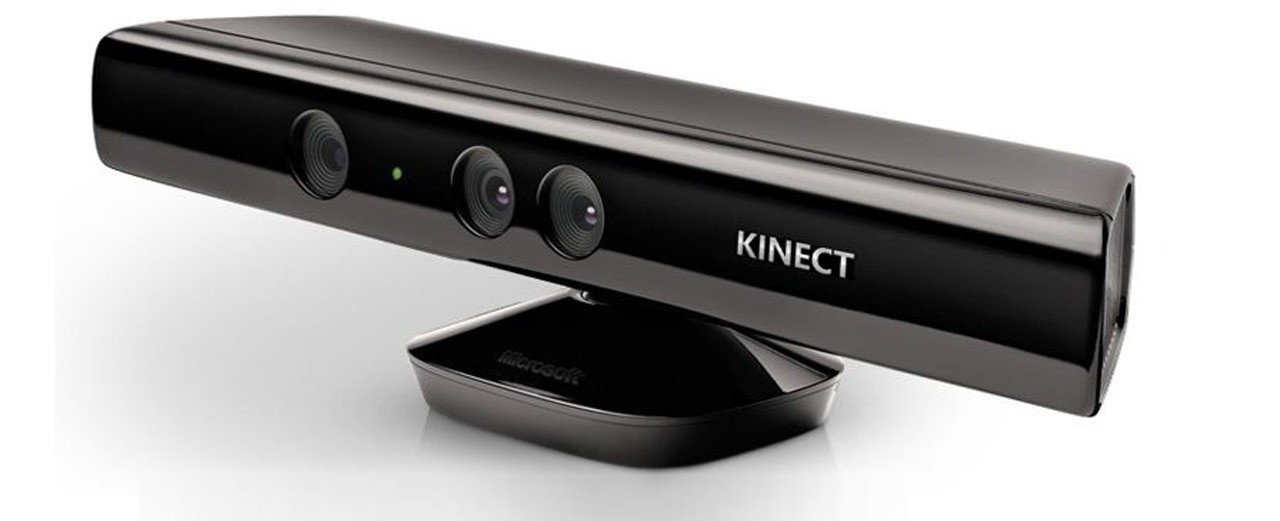
\includegraphics[scale=0.2]{kinect}
    \caption{Imagen que muestra la herramienta kinect.\protect\footnotemark}
    \label{figura-kinect}
  \end{figure}

  \footnotetext{ \url{https://www.vidaextra.com/hardware/kinect-esta-oficialmente-muerto}, Sergio Cejas}

  \item \textbf{Vincular la información a una escena}:  Lo que hace esta técnica es escanear las superficies del mundo real que se percibe por la camara y asignar coordenadas a dichas superficies, a cada una de estas coordenadas se puede asociar información virtual, como se puede ver en la Figura \ref{figura-scene}, en la que a algunas coordenadas se ha asignado un modelo 3D del muñeco de android, dicho modelo es la información virtual asociada a la coordenada.

  \begin{figure}[h]
    \centering
    
\includegraphics[scale=0.2]{scene}
    \caption{Imagen que muestra el reconocimiento de superficies de una escena y la asociación de información a una coordenada de esta escena.\protect\footnotemark}
    \label{figura-scene}
  \end{figure}

  \footnotetext{ \url{https://android.jlelse.eu/exploring-android-arcore-4463e15f928e}, Vortana Say}

  \item \textbf{Vincular la información a una coordenada del mundo real}: Se tendrá la información asignada a dicha coordenada del mundo, y gracias al sistema gps del dispositivo y otros sensores, permite que cuando dicha coordenada entre en el rango de visión del dispositivo, muestre la información asociada a esta, como se puede observar en la Figura \ref{figura-location}.

  \begin{figure}[h]
    \centering
    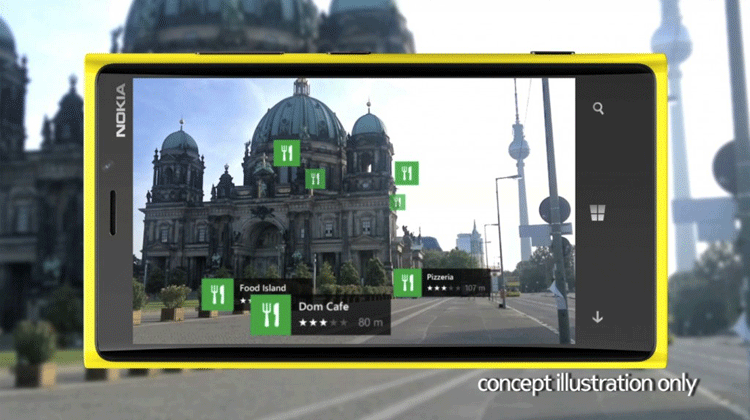
\includegraphics[scale=0.3]{location}
    \caption{Imagen que muestra la visualización de información asociada a coordenadas del mundo real.\protect\footnotemark}
    \label{figura-location}
  \end{figure}

  \footnotetext{ \url{https://www.gislounge.com/augmented-reality-digital-map-revolution/}, Nokia}

\end{itemize}

\section{Tecnologías de visualización de Realidad Aumentada}
En esta sección se abordará los diferentes tipos de pantalla que permiten la visualización en realidad aumentada \cite{billinghurst}, veremos categorizadas estas pantallas por la tecnología que utilizan, y también por la situación de dichas pantallas entre el usuario y el mundo real.\\

Existen diferentes tecnologías para utilizar en pantallas para visualización de realidad aumentada:
\begin{itemize}
  \item \textbf{Pantallas basadas en video}: Estas pantallas mediante procesos digitales combinan imágenes virtuales con video del mundo real. Estas pantallas son las más populares al estar en los dispositivos que usamos en el dia a dia como smartphones y tablets, como se puede ver en la Figura \ref{figura-pantalla-video}.

  \begin{figure}[h]
    \centering
    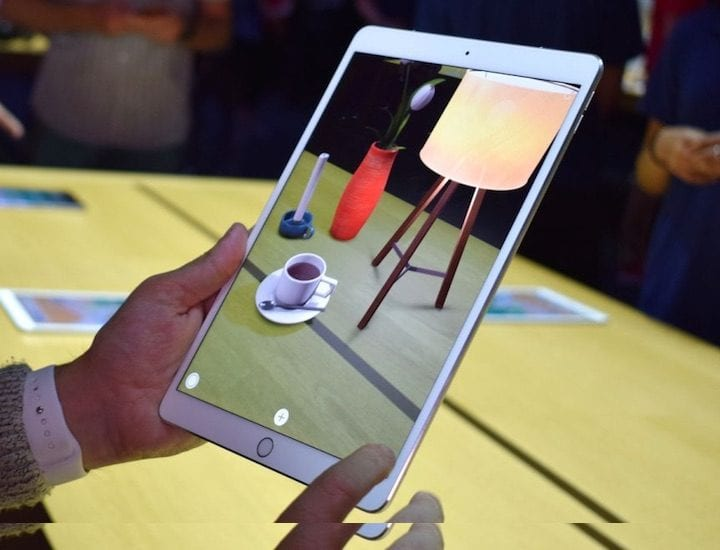
\includegraphics[scale=0.35]{video-screen}
    \caption{Imagen que muestra una tablet usando una aplicación de realidad aumentada.\protect\footnotemark}
    \label{figura-pantalla-video}
  \end{figure}

  \footnotetext{\url{https://urbantecno.com/tecnologia/arkit-realidad-aumentada-apple}, Eva Rodríguez de Luis}

  \newpage

  \item \textbf{Pantallas ópticas transparentes}: Estas pantallas mediante sistemas ópticos combinan imágenes virtuales con video del mundo real. Normalmente estas pantallas incluyen separadores de rayos, como un medio espejo, que permiten que en ese separador se vea la vista del mundo real a través del espejo, y los elementos virtuales añadidos, reflejados en el espejo, procedentes de una pantalla. En la Figura \ref{figura-pantalla-optica} se puede ver un esquema del funcionamiento de este tipo de pantallas.

  \begin{figure}[h]
    \centering
    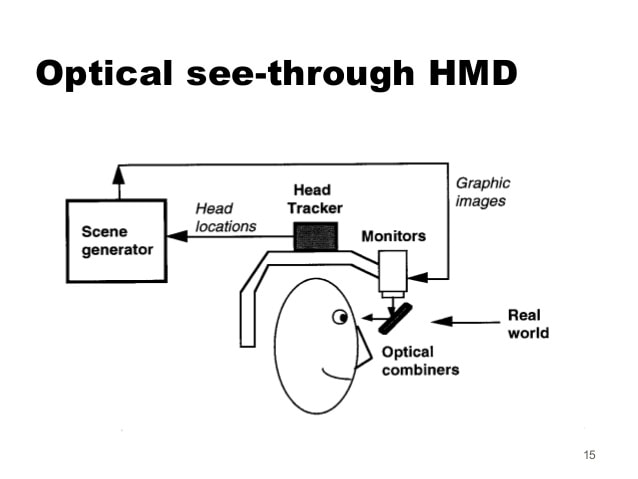
\includegraphics[scale=0.45]{optical-seethrough-screen}
    \caption{Imagen que muestra un esquema de como funcionan las pantallas opticas transparentes.\protect\footnotemark}
    \label{figura-pantalla-optica}
  \end{figure}

  \footnotetext{{\tt Augmented Reality ppt. [Diapositivas de Power Point]. Recuperado de }\\
  \url{https://www.slideshare.net/Khyati14Ganatra/augmented-reality-ppt-47315337}. {\tt Ganatra, K. (22 de abril de 2015).}}

  \newpage

  \item \textbf{Pantallas basadas en proyección}: Estas se encargan de proyectar las imágenes virtuales directamente sobre objetos del mundo real, como se puede ver en la Figura \ref{figura-pantalla-proyeccion}, esto combinado con el seguimiento de la posición del usuario y del objeto 3D, permite una aumentación interactiva. Por lo general, estos dispositivos suelen incluir un proyector montado en el techo o paredes.

  \begin{figure}[h]
    \centering
    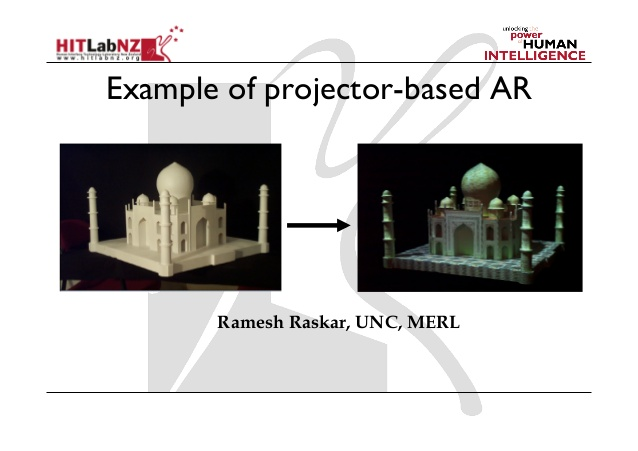
\includegraphics[scale=0.45]{projection-screen}
    \caption{Imagen que muestra como sobre un objeto se proyecta para conseguir una apariencia de objeto real.\protect\footnotemark}
    \label{figura-pantalla-proyeccion}
  \end{figure}

  \footnotetext{{\tt 2013 426 Lecture 2: Augmented Reality Technology. [Diapositivas de Power Point]. Recuperado de }\\
  \url{https://www.slideshare.net/marknb00/2013-426-lecture-2-augmented-reality-technology}. {\tt Billinghurst, M. (23 de julio de 2013).}}

  \item \textbf{Pantallas de ojo multiplexado}: Esta pantalla a diferencia de las anteriores no proporciona el mundo real con las imágenes virtuales ya mezcladas, si no que le proporciona al usuario ambas vistas y es el usuario el encargado de combinarlas mentalmente. Normalmente estas pantallas se suelen situar bastante cerca del ojo del usuario, para facilitar así la integración de los elementos virtuales que la pantalla muestra en el mundo real. Un ejemplo de visión con este tipo de pantallas se puede observar en la Figura \ref{figura-ojo-multiplexado}.

  \begin{figure}[h]
    \centering
    
\includegraphics[scale=0.2]{multiplexed-eye}
    \caption{Imagen que muestra como es llevar las Google Glass puestas.\protect\footnotemark}
    \label{figura-ojo-multiplexado}
  \end{figure}

  \footnotetext{ \url{https://www.youtube.com/watch?v=d-y3bEjEVV8}, Phandroid}

\end{itemize}

\newpage

\begin{flushleft}
Otra forma de categorizar los tipos de pantalla puede ser por la situación de la pantalla entre el usuario y el mundo real:
\end{flushleft}

\begin{itemize}
  \item \textbf{Head-attached displays}: Son dispositivos que van colocados en al cabeza del usuario, y que pueden ser desde el tamaño de un casco al tamaño de unas gafas.

  \item \textbf{Hand-held display}: Son dispositivos que el usuario puede sujetar con las manos, generalmente serán smartphones y tablets.

  \item \textbf{Spatial displays}: Suelen ser pantallas que están colocadas en un dispositivo o habitación, por lo que no permiten mucha movilidad.

\end{itemize}

\begin{flushleft}
Algunos ejemplos de Head-attached displays:
\end{flushleft}

\begin{itemize}
  \item \textbf{Hololens}: Este dispositivo entraría dentro de las pantallas ópticas transparentes, básicamente tienen unas lentes transparentes que permiten ver el mundo real, pero a la vez en estas se proyectan hologramas que se integran perfectamente con el mundo real gracias a los sensores que las gafas llevan integrados \cite{hololens}.

  \begin{figure}[h]
    \centering
    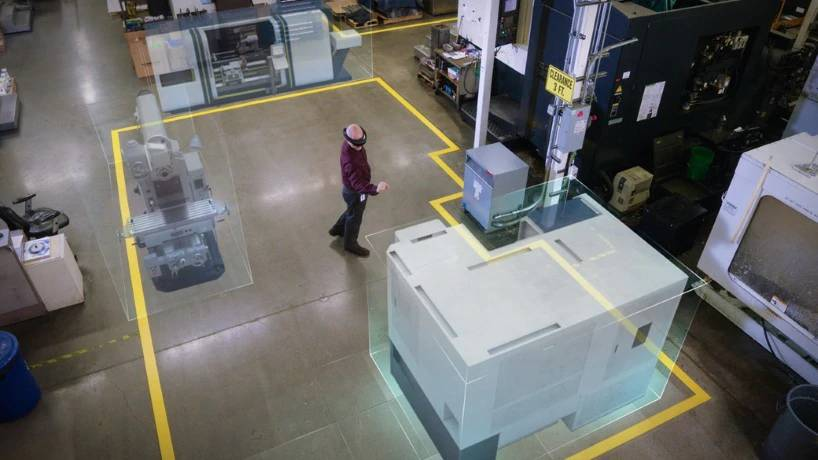
\includegraphics[scale=0.33]{head-hololens}
    \caption{Imagen que las gafas Hololens.\protect\footnotemark}
    \label{figura-hololens}
  \end{figure}

  \footnotetext{ \url{https://www.microsoft.com/es-es/hololens/commercial-overview}, Microsoft}

  \newpage

  \item \textbf{Google glass}: Este dispositivo entraría dentro de las pantallas de ojo multiplexado, son unas gafas que tienen un pequeño espejo semi-reflectivo en el que se muestran las imágenes, que al estar cerca del ojo superpone la información sobre el mundo real \cite{likamwa}.

  \begin{figure}[h]
    \centering
    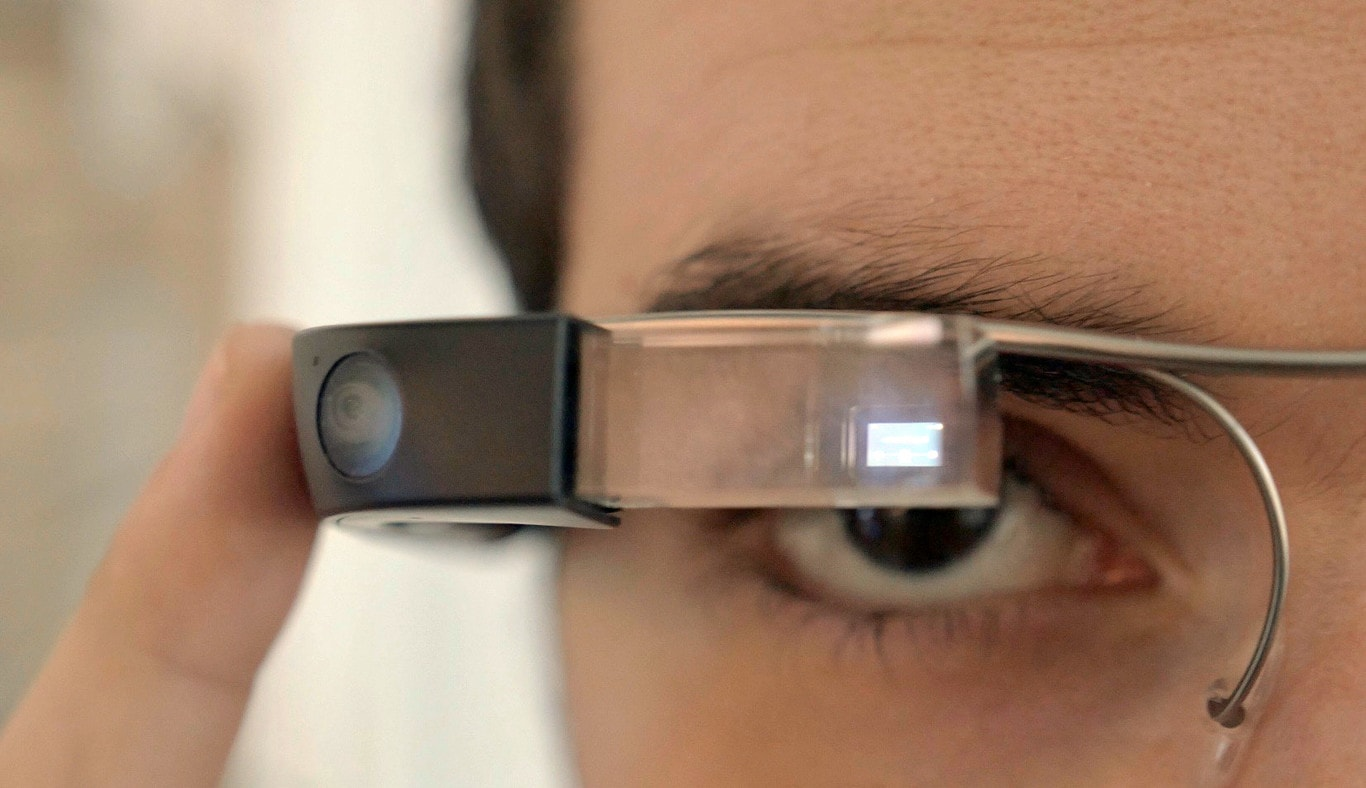
\includegraphics[scale=0.21]{head-googleglass}
    \caption{Imagen que las gafas Google Glass.\protect\footnotemark}
    \label{figura-googleglass}
  \end{figure}

  \footnotetext{ \url{https://www.xataka.com/realidad-virtual-aumentada/no-estaban-muertas-google-glass-enterprise-salen-a-la-venta-y-para-esto-sirven-en-2017}, Xataka}

\newpage

  \item \textbf{Meta glasses}: Este dispositivo entraría dentro de las pantallas ópticas transparentes, funciona igual que las Hololens, con la diferencia de que necesitan estar conectadas a un ordenador para llevar a cabo el procesamiento gráfico \cite{meta-vision}.

  \begin{figure}[h]
    \centering
    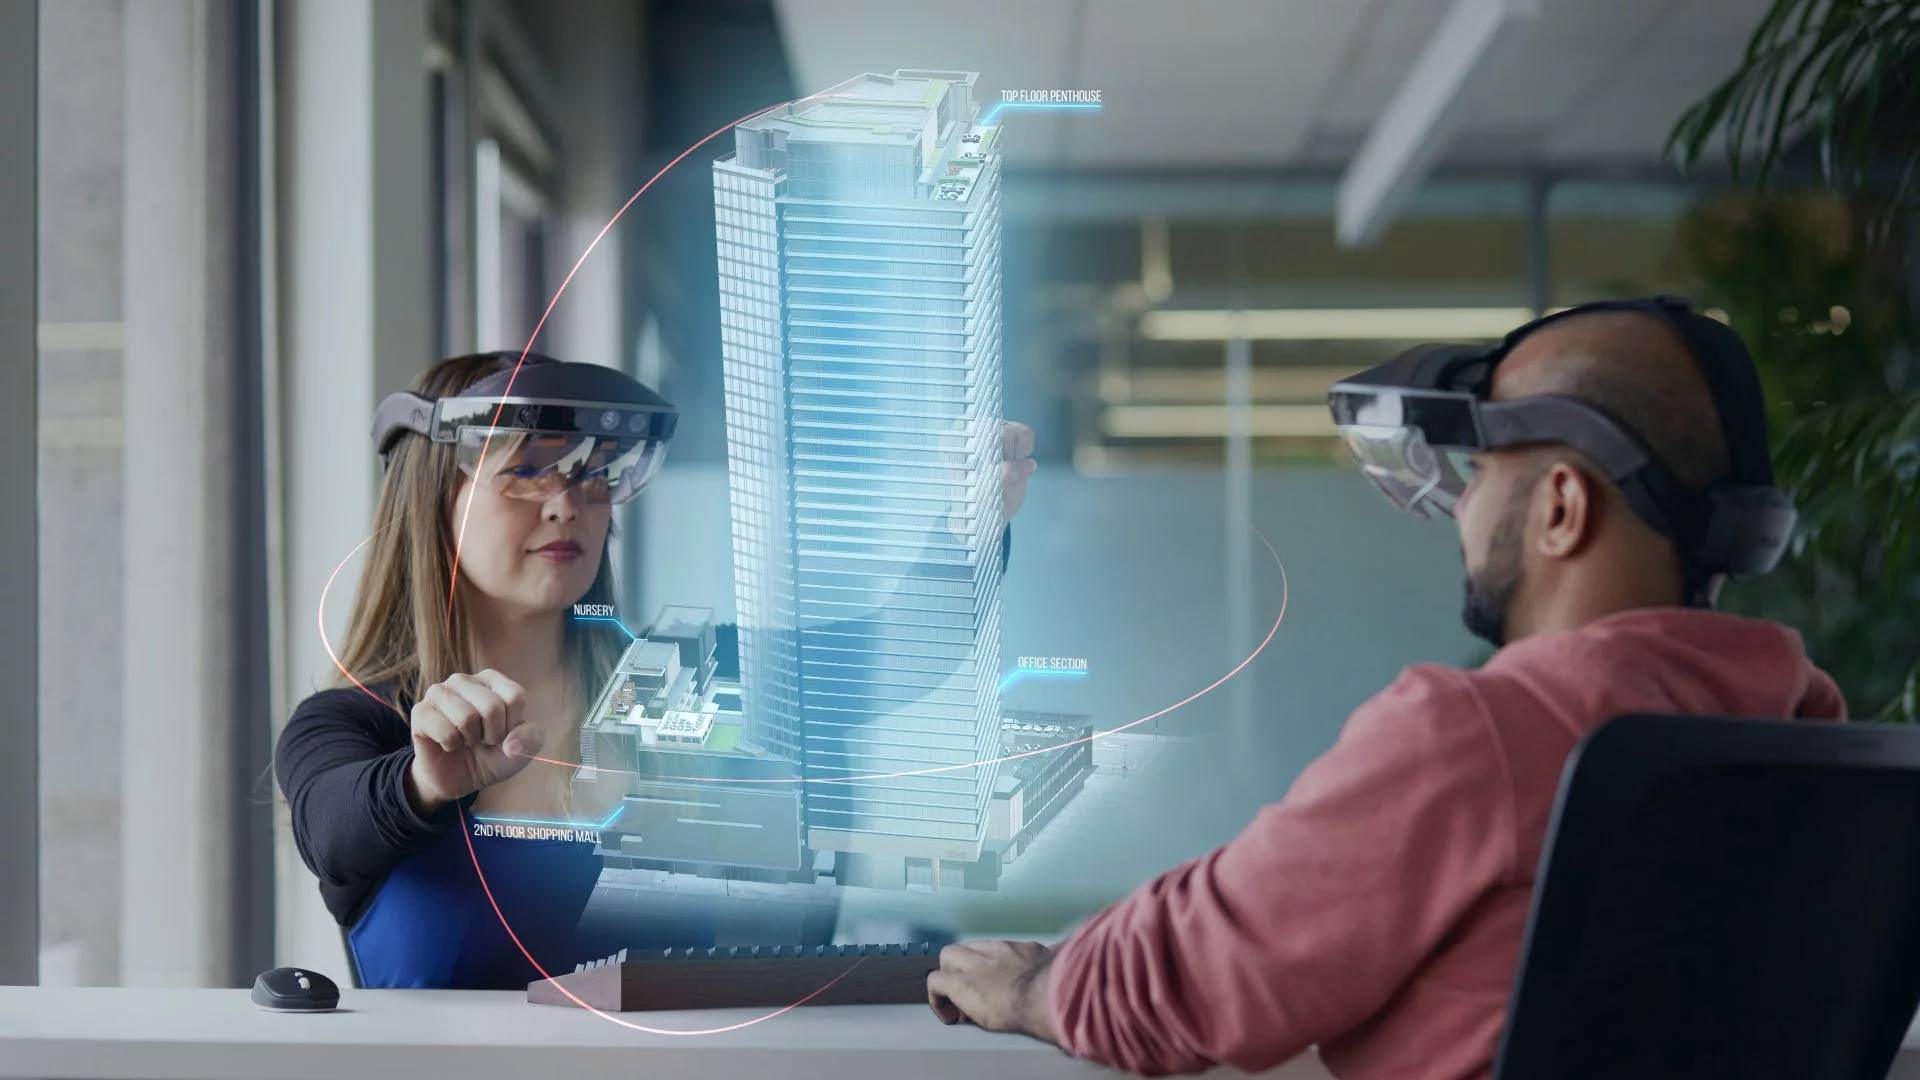
\includegraphics[scale=0.15]{head-metaglasses}
    \caption{Imagen que las gafas Meta Glasses.\protect\footnotemark}
    \label{figura-metaglasses}
  \end{figure}

  \footnotetext{ \url{http://www.metavision.com/}, Meta}

  \newpage

  \item \textbf{Magic Leap}: Este dispositivo entraría dentro de las pantallas ópticas transparentes, el funcionamiento de estas gafas es algo especial, dado que la pantalla es capaz de crear campos de luz como los que percibimos del mundo real, para que la visualización de un objeto 3D sea más natural y no canse la vista \cite{magic-leap}.

  \begin{figure}[h]
    \centering
    
\includegraphics[scale=0.28]{head-magicleap}
    \caption{Imagen que las gafas Magic Leap.\protect\footnotemark}
    \label{figura-magicleap}
  \end{figure}

  \footnotetext{ \url{https://elpais.com/tecnologia/2017/12/20/actualidad/1513784616_903835.html}, El Pais}

  \item \textbf{Mira Headset}: Este dispositivo entraría dentro de las pantallas ópticas transparentes, básicamente dispone de unas gafas con cristal reflectivo y un hueco para colocar un smartphone, por lo que se puede ver a través, pero se ve superpuesta la imagen que muestra el dispositivo móvil gracias a la aplicación de la propia empresa \cite{mira-ar}.

  \begin{figure}[h]
    \centering
    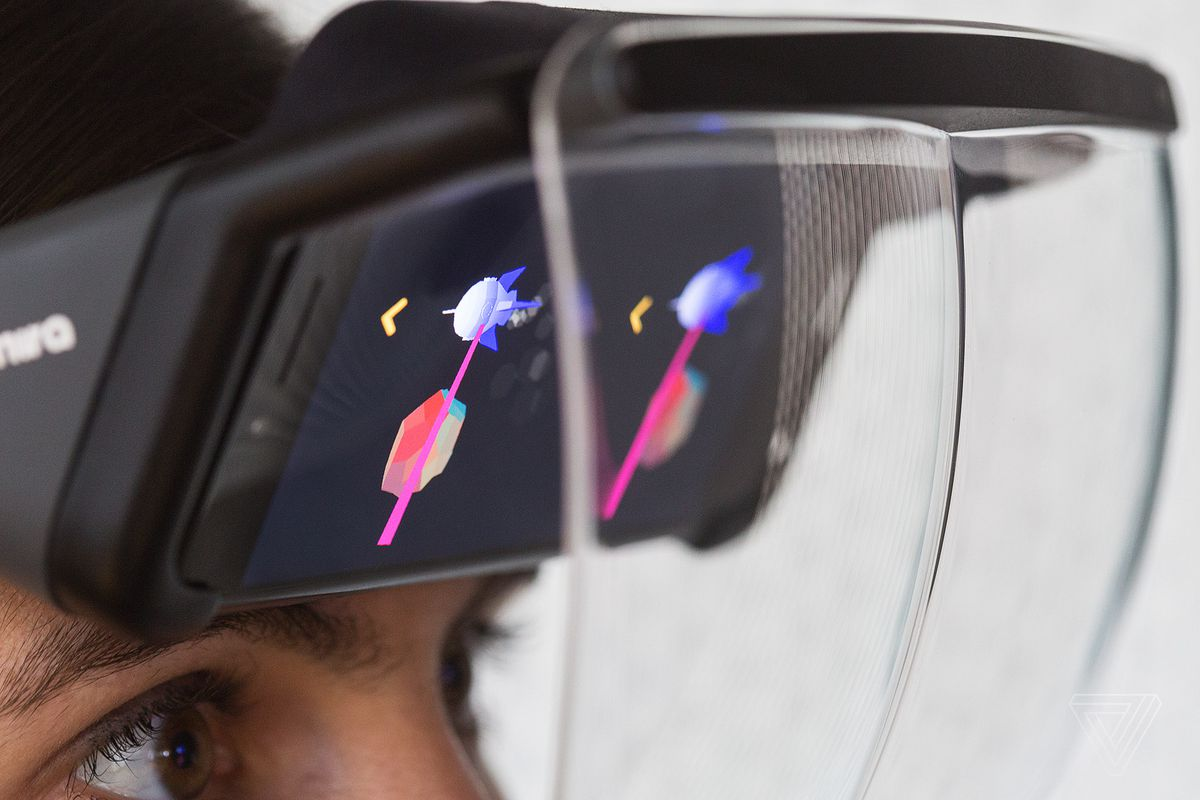
\includegraphics[scale=0.15]{head-miraheadset}
    \caption{Imagen que las gafas Mira Headset.\protect\footnotemark}
    \label{figura-miraheadset}
  \end{figure}

  \footnotetext{ \url{https://www.theverge.com/2017/7/18/15948700/mira-prism-iphone-augmented-reality-headset-hands-on-announce}, The Verge}

\end{itemize}

\section{Desarrollo de realidad aumentada}
El desarrollo de aplicaciones que incorporen elementos de realidad aumentada se puede llevar a cabo de dos maneras, usando un SDK o utilizando herramientas de autor. Los SDK ofrecen una librería de código que permite acceder a las funciones de realidad aumentada, como por ejemplo, detectar una imagen y asociar información a esta. Por otro lado las herramientas de autor permiten asociar la información a elementos del mundo real de una forma sencilla, como puede ser mediante una interfaz gráfica. Los SDK tienen la ventaja de ofrecer mas libertad, mientras que las herrmientas de autor ofrecen facilidad en el desarrollo.

\subsection{Librerías}
\begin{itemize}
  \item \textbf{ARKit}: Es la librería creada por Apple para llevar la realidad aumentada a los dispositivos iOS que dispongan de la versión 11 o superior, hace uso de tecnologías similares a ARCore para conocer la posición del dispositivo, detectar superficies horizontales, verticales e irregulares y para conocer las condiciones de luz del entorno \cite{arkit}.

  \item \textbf{Vuforia}: Es un SDK de realidad aumentada muy popular que permite desarrollar aplicaciones tanto para Android como para iOS, su funcionamiento consiste en introducir modelos virtuales en diferentes targets u objetivos, que serán detectados por la camara. Estos objetivos pueden ser imágenes planas como la página de una revista o una fotografía sobre las que se puede colocar un modelo virtual, objetos con diferentes superficies planas, en las que cada superficie plana se considera un objetivo diferente, o modelos que a partir de un modelo 3D permite reconocer uno real a través de la cámara, y utilizarlo como objetivo, por ejemplo coches o juguetes \cite{vuforia}.

  \item \textbf{EasyAR}: Es un SDK de realidad aumentada que permite desarrollar aplicaciones tanto para Android como para iOS, contiene varias API que permiten programar en c, c++, java en caso de hacer la aplicación para Android y swift en caso de hacer la aplicación para iOS, permite la detección de imágenes planas, es decir, fotos o páginas de revista entre otros sobre las que se puede colocar el modelo virtual, permite la detección de varios objetivos simultáneamente y que el reconocimiento de objetivos se haga en la nube, también permite el seguimiento de objetos 3D \cite{easyar}.

  \item \textbf{Wikitude}: Es un SDK de realidad aumentada muy reconocida que permite desarrollar aplicaciones tanto para Android, iOS y smartglasses. Incluye en un mismo SDK ARCore y ARKit con su propia plataforma. Permite el reconocimiento de objetos, de imágenes, sobre las que permite colocar un modelo virtual, también permite la geolocalización y el reconocimiento en la nube \cite{wikitude}.
\end{itemize}


\subsection{Herramientas de autor}
\begin{itemize}
  \item \textbf{AR Studio}: Es una herramienta desarrollada por Facebook que te permite crear efectos/elementos que se pueden aplicar al mundo real cuando usas la cámara, es capaz de seguir varios puntos en una cara y de detectar superficies planas, lo que permite aplicar dichos efectos/elementos a esos puntos. La forma de crear estas experiencias de realidad aumentada es mediante un editor gráfico, lo que facilita el proceso \cite{ar-studio}.

  \begin{figure}[h]
    \centering
    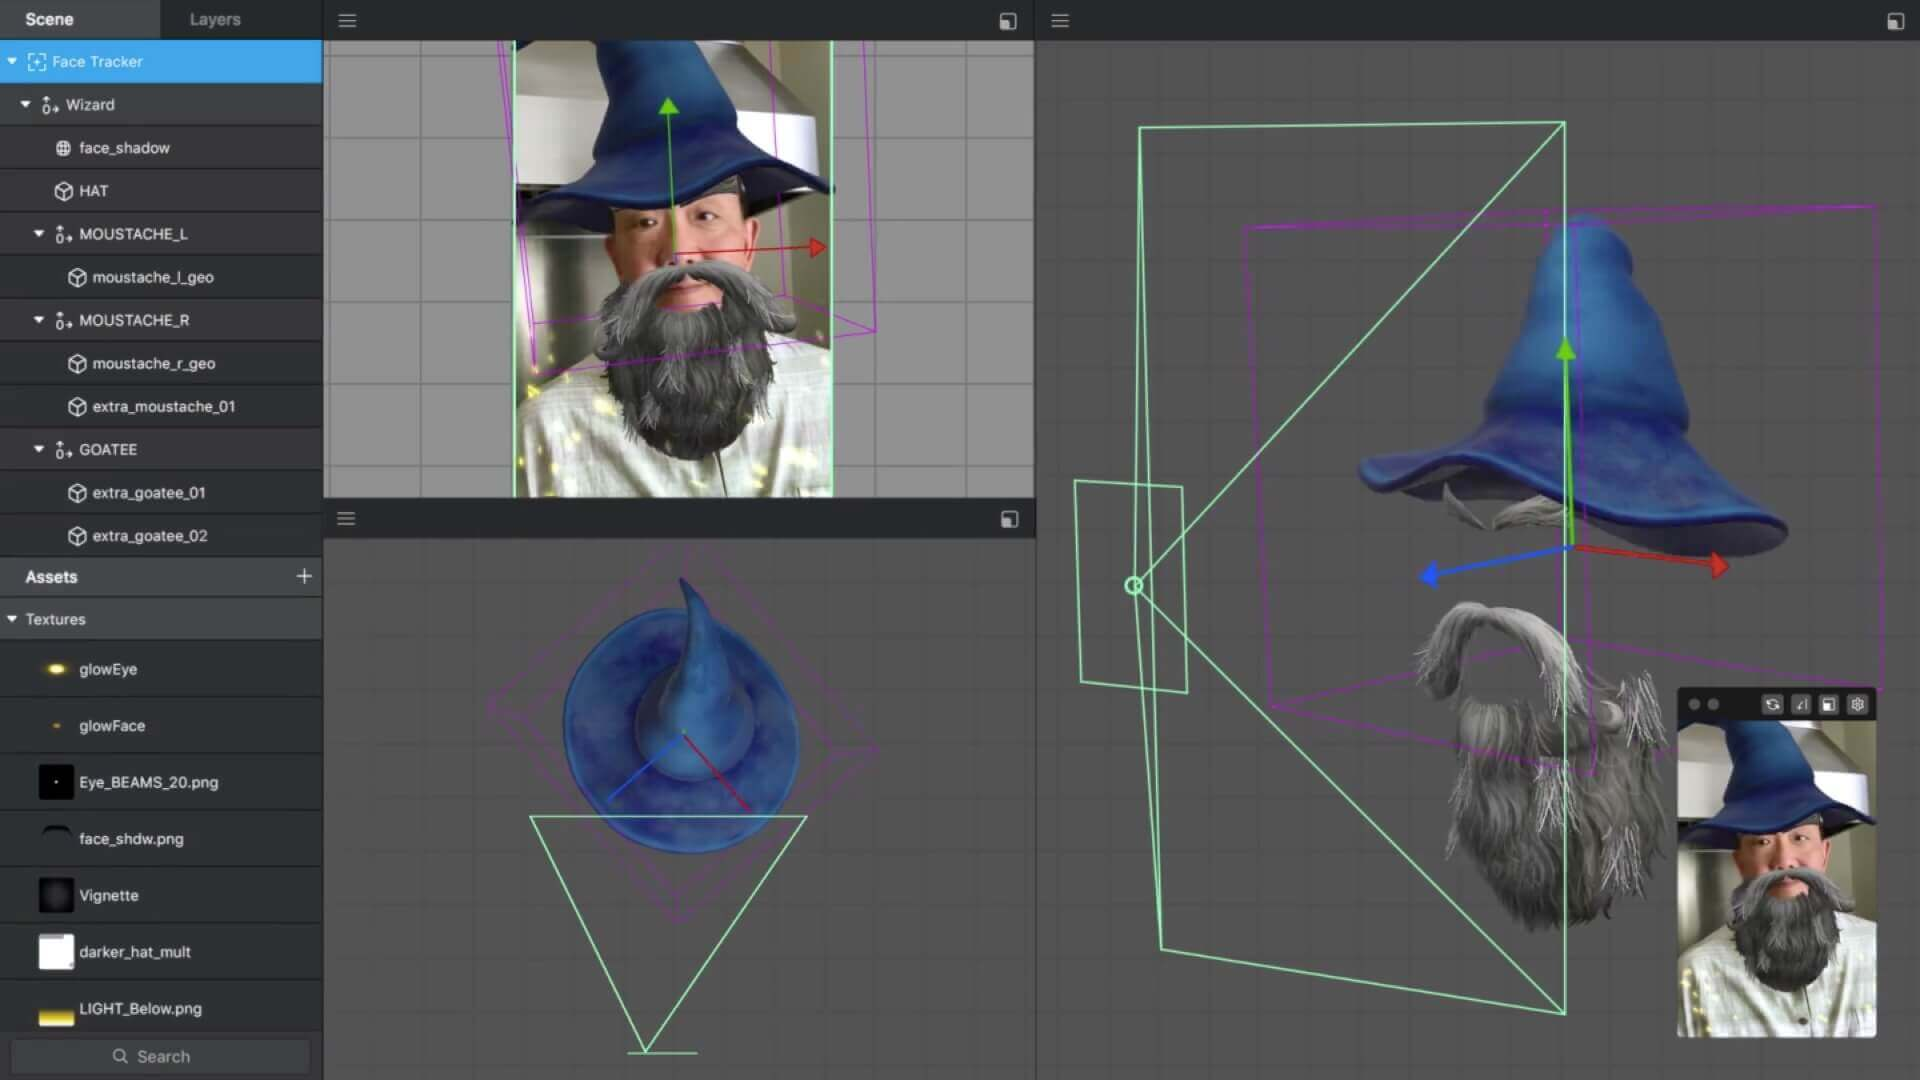
\includegraphics[scale=0.17]{head-ar-studio}
    \caption{Imagen que muestra el editor AR Studio.\protect\footnotemark}
    \label{figura-arstudio}
  \end{figure}

  \footnotetext{ \url{https://marketingland.com/hands-facebooks-ar-studio-create-snapchat-like-camera-effects-212664}, Marketing Land}

  \newpage

  \item  \textbf{Layar}: Es una herramienta desarrollada por la propia empresa Layar, que permite de una forma sencilla crear experiencias de realidad aumentada a partir de una imagen que tu cargas, y la forma de crear esa experiencia es con un editor gráfico. Por ejemplo, puedes poner la imagen de una tarjeta de felicitación y con el editor crear los elementos de realidad aumentada que surgirán a partir de la tarjeta \cite{layar}.
\end{itemize}

\begin{figure}[h]
  \centering
  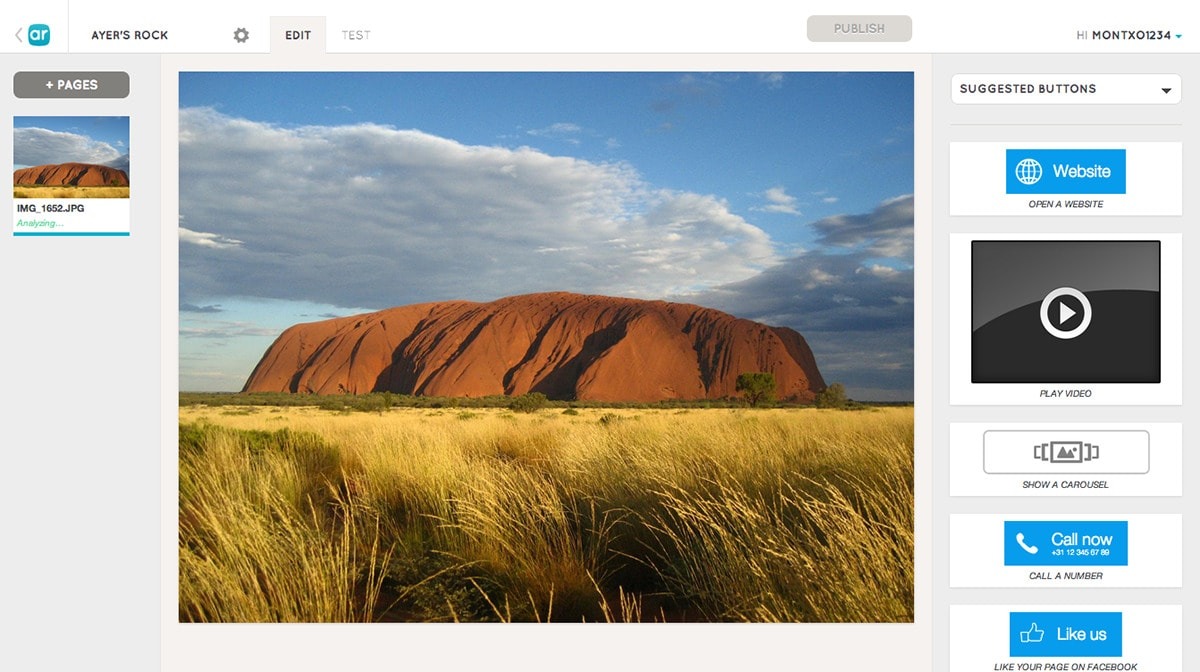
\includegraphics[scale=0.3]{head-layar}
  \caption{Imagen que muestra el editor Layar Creator.\protect\footnotemark}
  \label{figura-layar}
\end{figure}

\footnotetext{ \url{https://www.behance.net/gallery/15241153/Layar-Creator-20}, Behance}

\subsection{ARCore}
Este SDK concreto es el que se va a utilizar en el desarrollo del proyecto, por lo tanto, se expondrán con mayor profundidad sus características.\\

Es la librería creada por Google para llevar la realidad aumentada a los dispositivos android que dispongan de la versión 7 o superior, esta librería se basa en el uso de tres tecnologías, motion tracking para que el telefono conozca cuál es su posición relativa al mundo real, environment understanding para que el teléfono detecte la posición y tamaño de superficies horizontales planas y light estimation para que el teléfono pueda conocer las condiciones de luz del entorno.\\

La tecnología motion tracking que utiliza le permite a través de la camara identificar puntos interesantes del mundo y ver cómo estos puntos se mueven con el tiempo. Y combinando el movimiento de dichos puntos y los sensores del teléfono puede determinar la posición y orientación del teléfono conforme este se mueve por el espacio.\\

Además de estos puntos de interés, ARCore detecta superficies planas, que junto con la estimación de luz le permiten construir su propia representación del mundo.\\

Esta representación del mundo permite situar información como objetos, anotaciones, etc. que se integra perfectamente en el mundo real \cite{arcore}.\\

Elementos destacables de ARCore:

\begin{itemize}
  \item \textbf{Augmented Images}: Permite a una aplicación que hace uso de la tecnología ARCore, detectar imágenes 2D en el mundo real y sabe las posiciones de estas, es decir, sabe dónde está cada imagen escaneada con respecto al mundo real, por lo que puedes moverte, y la aplicación seguirá teniendo el conocimiento de que está ahí situada esa imagen. Y a una imagen puedes asociar elementos 3D, que se situarán donde el desarrollador indique con respecto a la posición de la imagen a la que están asociados, por lo que, una vez detectada puedes moverte que los elementos 3D mostrados seguirán en esa posición aunque la imagen desaparezca de cámara, ya que, como se ha explicado mantiene la posición de dicha imagen, y por tanto, de sus elementos asociados con respecto al mundo real. No permite el reconocimiento de una imagen en movimiento, por lo que una vez la imagen se vuelva a parar, volvera a reconocerla y mostrar los elementos 3D asociados a ella. Se puede utilizar desarrollando con Android, Android NDK, Unity y Unreal Engine \cite{arcore-augmented-images}.

  \item \textbf{Cloud Anchors}: Permite a una aplicación que hace uso de la tecnología ARCore, compartir Anchors entre distintos dispositivos. Un Anchor describe una ubicación fija y una orientación en el mundo real, por lo que, se puede usar para entonces enlazar objetos a ese anchor, de forma que ese objeto tomará esa posición en el mundo y esa orientación y no se modificará, aportando así una mayor sensación de realismo \cite{arcore-anchors}. Por tanto, al compartir estos anchors, si desde otro dispositivo escaneas la misma escena, va a ser capaz de posicionar dicho anchor en el dispositivo actual, y mostrar los elementos enlazados a dicho anchor en el dispositivo, permitiendo así crear experiencias compartidas. Este componente está disponible tanto para Android como para iOS, de forma que un juego desarrollado para diferentes sistemas operativos pueda compartir esta información, fundamental para las experiencias de realidad aumentada compartidas. Se puede utilizar desarrollando con Android, Android NDK, Unity y Unreal Engine \cite{arcore-cloud-anchors}.

  \item \textbf{Sceneform}: Permite a una aplicación que utiliza ARCore trabajar con dicha tecnología sin necesidad de tener conocimientos acerca de gráficos 3D y OpenGL. Sceneform añade un plugin a Android Studio que permite importar, ver y construir modelos 3D, y también añade una API de alto nivel para los gráficos de escena, todo esto integrable de forma sencilla con ARCore de forma que es sencillo hacer aplicaciones de realidad aumentada \cite{arcore-sceneform}.

\end{itemize}

Actualmente ARCore tiene soporte para desarrollo en las siguientes plataformas:

\begin{itemize}
  \item \textbf{Android}: Se utilizará el framework “Android Studio”, y el lenguaje Java.

  \item \textbf{Android NDK (Kit de desarrollo nativo)}: Se utilizará el framework “Android Studio”, y el lenguaje C o C++. Android NDK consiste en un conjunto de herramientas que te permiten utilizar código C o C++ en aplicaciones Android, de forma que, por ejemplo, puedes utilizar bibliotecas que ya tenias, mejorar el rendimiento de la aplicación o conectar una aplicación entre plataformas \cite{ndk}.

  \item \textbf{iOS}: ARCore permite que mientras se desarrolla utilizando ARKit, mediante la SDK que proporcionan puedas utilizar anchors que otro dispositivo ha creado, usando la característica “Cloud Anchor”, o crear esos anchors y compartirlos.

  \item \textbf{Unity}: Permite el desarrollo de videojuegos con Unity utilizando el SDK de ARCore para esta plataforma, la programación de los scripts característicos de Unity se llevará a cabo utilizando el lenguaje C# o UnityScript, lenguaje que fue creado con JavaScript como base \cite{unity-scripting}.

  \item \textbf{Unreal Engine}: Permite el desarrollo de videojuegos con Unreal Engine utilizando el SDK de ARCore para esta plataforma, la programación en Unreal se lleva a cabo utilizando el lenguaje C++ \cite{unreal}.

  \item \textbf{Web}: Permite el desarrollo web utilizando Realidad Aumentada, de forma que usando la librería javascript “three.ar.js”, y un navegador especial para realidad aumentada que ellos proporcionan, se puede utilizar la realidad aumentada en tecnologías web \cite{arcore-web}.
\end{itemize}

\subsection{Tabla comparativa de librerías}
%%%%%%%%%%%%%%%%%%%%%%%%%%%%%%%%%%%%%%%%%%% TABLA COMPARATIVA LIBRERIAS %%%%%%%%%%%%%%%%%%%%%%%%%%%%%%%%%%%%%%%%%%%%%%%%
\begin{table}[h]
  \begin{center}
    \begin{tabular}{|p{1.5cm}|p{2.3cm}|p{1.7cm}|p{2.2cm}|p{2cm}|p{2cm}|}

      \hline
        \rowcolor{Gray} \textbf{Librería}
        & \textbf{Plataformas compatibles}
        & \textbf{Licencia}
        & \textbf{Detección de imágenes}
        & \textbf{Seguimiento de imagen}
        & \textbf{Experiencia inter-dispositivo}\\

      \hline
      ARKit
      & iOS, Xcode
      & Libre
      & Si
      & Si
      & Si\\

      \hline
      Vuforia
      & Android, iOS, Unity
      & Comercial y Libre
      & Si
      & Si
      & No\\

      \hline
      EasyAR
      & Android, iOS, Unity
      & Comercial y Libre
      & Si
      & Si
      & No\\

      \hline
      Wikitude
      & Android, iOS, Titanium, Xamarin, Cordova, Unity
      & Comercial
      & Si
      & Si
      & No\\

      \hline
      ARCore
      & Android, Unity, Unreal Engine, Android Studio, iOS
      & Libre
      & Si
      & No
      & Si\\

      \hline

    \end{tabular}

    \caption{Tabla comparativa de librerías.}
    \label{tabla-librerias}

  \end{center}
\end{table}

\newpage

\section{Interfaces tangibles}
A la hora de interactuar con una aplicación de realidad aumentada para dispositivos móviles hay dos opciones, se puede interactuar mediante la pantalla del dispositivo, o mediante el uso de elementos físicos. Estos elementos físicos son considerados interfaces tangibles, ya que nos permiten interactuar con la aplicación mediante la manipulación de dichos elementos físicos.\\

Las interfaces tangibles aportan una experiencia mucho mas natural para el ser humano, ya que el ser humano esta acostumbrado a interactuar con elementos físicos y le resulta mucho mas natural que realizar toques en una pantalla, que si bien es sencillo de hacer, no resulta tan realista para el usuario.\\

Las interfaces tangibles son interfaces de usuario mediante las cuales el usuario interactúa con la información digital a través del entorno físico \cite{ullmer}.\\

El mayor ejemplo de interfaz tangible es el ratón, en el caso de la realidad aumentada la interfaz tangible consiste en un elemento, que al entrar dentro del rango de la cámara se convierte en un elemento que puede modificar la información virtual que se está mostrando en la pantalla.\\

Como ejemplo de interfaces tangibles en realidad mixta tenemos los “Motion controllers” del kit “Microsoft Mixed Reality”, son dos mandos que al ser reconocidos por los sensores del casco permiten modificar elementos virtuales \cite{windows-mixed-reality}.\\

\begin{figure}[h]
  \centering
  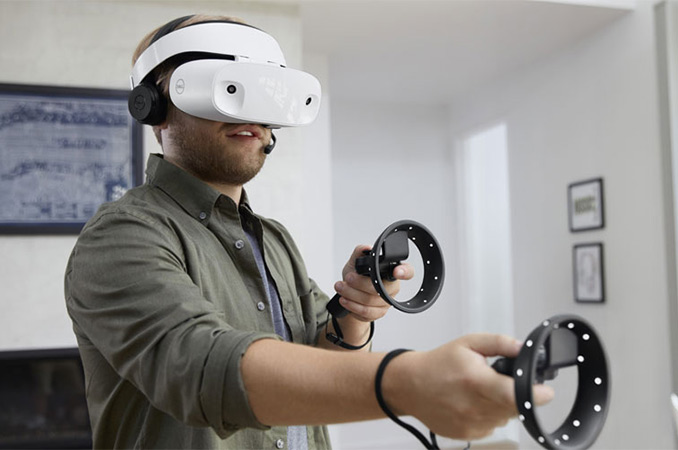
\includegraphics[scale=0.3]{windows-mixed-reality}
  \caption{Imagen que muestra los "Motion controllers".\protect\footnotemark}
  \label{figura-windowsmixedreality}
\end{figure}

\footnotetext{ \url{https://www.anandtech.com/show/11841/dells-visor-windows-mixed-reality-headset}, Anandtech}


Como ejemplo de interfaces tangibles en realidad aumentada tenemos ARtalet, es un proyecto que permite reconocer la posición de un ratón puntero por unas pegatinas en la punta de éste, y recibe señales de los botones del ratón. Mediante los botones del ratón y ese puntero que reconoce la camara son capaces de manipular otros elementos virtuales que se habían situado en el entorno real que la cámara percibe \cite{ha}.\\

\begin{figure}[h]
  \centering
  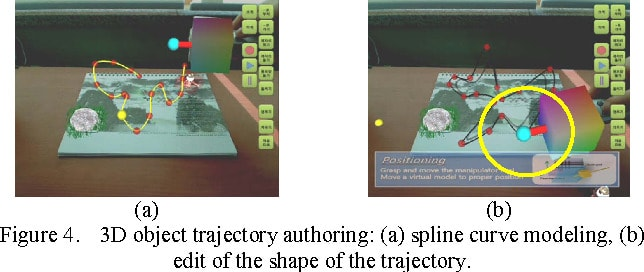
\includegraphics[scale=0.5]{artalet}
  \caption{Imagen que muestra la interfaz tangible utilizada en ARTalet.\protect\footnotemark}
  \label{figura-artalet}
\end{figure}

\footnotetext{{\em ARtalet: tangible user interface based immersive augmented reality authoring tool for Digilog book. In Ubiquitous Virtual Reality (ISUVR)}, 2010 International Symposium on (pp. 40-43). IEEE. Ha, T., Woo, W., Lee, Y., Lee, J., Ryu, J., Choi, H., & Lee, K. (2010, July).}

%%%%%%%%%%%%%%%%%%%%%%%%%%%%%%%%%%%%%%%%%%% ESTUDIO DE MERCADO APPS AR %%%%%%%%%%%%%%%%%%%%%%%%%%%%%%%%%%%%%%%%%%%%%%%%%

\section{Estudio de mercado sobre aplicaciones que hacen uso de realidad aumentada}

Este estudio de mercado explora los diferentes usos que se da a la realidad aumentada en aplicaciones actualmente, por lo que se listarán los tipos de uso:

\begin{itemize}
  \item \textbf{Puzzle-Perspectiva}: Consisten en puzles que se resuelven utilizando la perspectiva, moviéndote alrededor del puzle que se m uestra en 3D sobre una superficie plana.
  \begin{itemize}
    \item \textbf{Mazelith}: Este juego ha utilizado el 3D para que en función del lugar desde el que visualices la pieza se pueda resolver el puzle, uniendo la vía por la que circula la luz. La ventaja que le da la realidad aumentada a este juego es el aumento de realismo, ya que ahora lo juegas físicamente moviéndote alrededor en lugar de mover la escena con los dedos para encontrar la perspectiva adecuada.

    \begin{figure}[h]
      \centering
      
\includegraphics[scale=0.13]{mazelith}
      \caption{Imagen que muestra el juego Mazelith.\protect\footnotemark}
      \label{figura-mazelith}
    \end{figure}

    \footnotetext{ \url{https://itunes.apple.com/es/app/mazelith/id1328826457?mt=8}, Monogrid}
  \end{itemize}

  \item \textbf{Shooter}: Consisten en enemigos virtuales que se muestran en el espacio físico de tu alrededor, a los cuales tienes que disparar para conseguir más puntuación.

  \begin{itemize}
    \item \textbf{Ghosts’n guns - AR Shooter}: Este juego utiliza el concepto de shooter clásico, en el que te aparecen enemigos y tienes que dispararles hasta derrotarlos. Utiliza la realidad aumentada de forma que ahora en lugar de estar todo dentro de la pantalla, tu eres el que dispara en la vida real y tienes que apuntar con el móvil bien para acertar, introduciendo un mayor realismo en el juego.

    \begin{figure}[h]
      \centering
      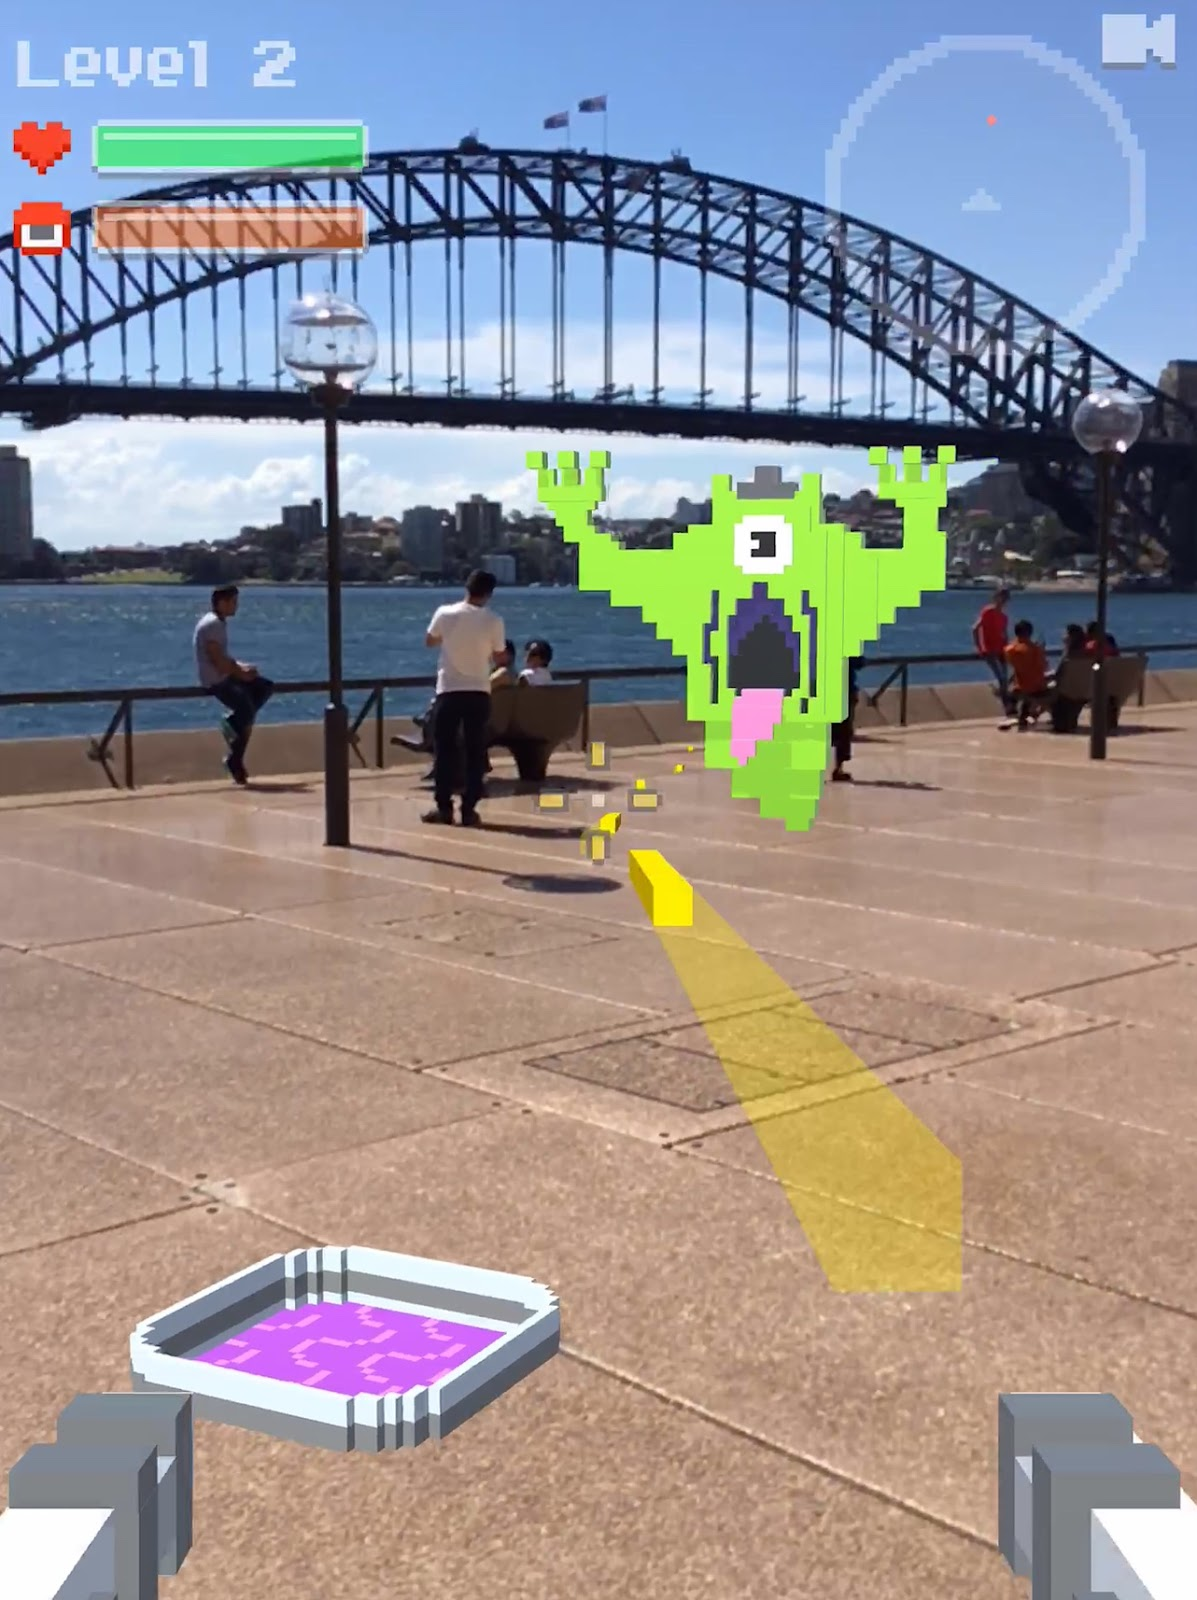
\includegraphics[scale=0.12]{ghostsguns}
      \caption{Imagen que muestra el juego Ghosts'n guns.\protect\footnotemark}
      \label{figura-ghosts-guns}
    \end{figure}

    \footnotetext{ \url{https://itunes.apple.com/us/app/ghosts-n-guns-ar/id1312708394?mt=8}, Turbo Chilli Pty Ltd}
  \end{itemize}

  \item \textbf{Mapa 3D}: Consisten en juegos que sitúan un mapa sobre una superficie plana, y la dinámica del juego es la misma que si fuera en 2D en la pantalla, pero ahora recibes nuevas perspectivas en 3D.

  \begin{itemize}
    \item \textbf{Siege Breakers}: Este juego consiste en demoler edificios colocando explosivos estratégicamente. La aplicación de realidad aumentada en este caso permite una mejor experiencia de usuario, ya que resulta más sencillo moverse alrededor del edificio y por tanto la decisión de dónde colocar el explosivo será más sencilla y efectiva.

    \begin{figure}[h]
      \centering
      
\includegraphics[scale=0.1]{siegebreakers}
      \caption{Imagen que muestra el juego Siege Breakers.\protect\footnotemark}
      \label{figura-siege-breakers}
    \end{figure}

    \footnotetext{ \url{https://itunes.apple.com/es/app/siege-breakers/id1276405526?mt=8}, Halfbrick Studios}
  \end{itemize}

  \newpage

  \item \textbf{Juegos de mesa}: Consisten en un juego de mesa, que en lugar de mostrarse en la pantalla, se sitúa en una superficie plana, por ejemplo una mesa, dando una sensación de jugar un juego de mesa real.

  \begin{itemize}
    \item \textbf{Chess+ AR}: Este juego consiste en situar un tablero de ajedrez en una superficie plana del mundo real, y jugar una partida de ajedrez. La realidad aumentada permite situar el tablero en el mundo real, dando la sensación de ser un juego real, aunque físicamente no esté.

    \begin{figure}[h]
      \centering
      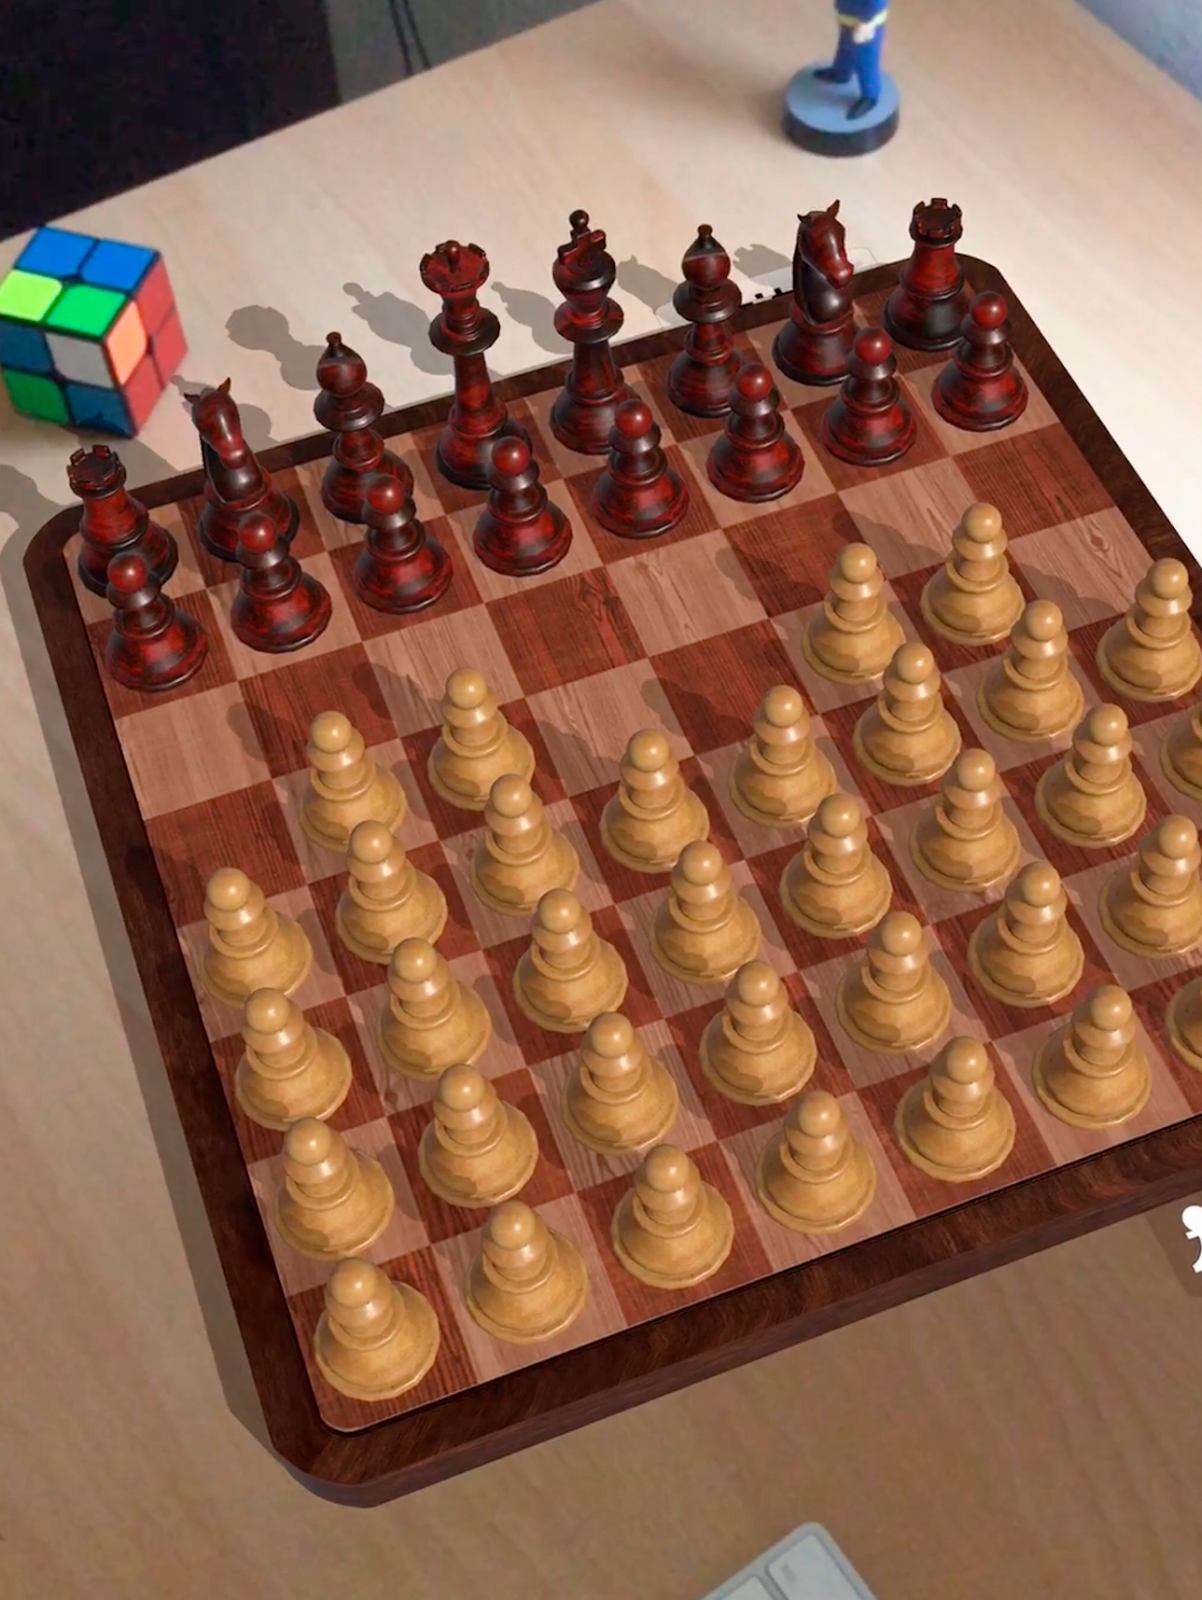
\includegraphics[scale=0.1]{chess}
      \caption{Imagen que muestra el juego Chess+ AR.\protect\footnotemark}
      \label{figura-siege-breakers}
    \end{figure}

    \footnotetext{ \url{https://itunes.apple.com/us/app/chess-ar/id1273831380?mt=8}, Jorge Moreno Aguilera}
  \end{itemize}

  \newpage

  \item \textbf{Exploración}: Consisten en aprovechar el conocimiento de la posición del dispositivo en el entorno físico, y que se almacena todas las superficies a tu alrededor, de forma que se aprovechan todas estas superficies registradas, por ejemplo, enterrando cofres del tesoro, y en el siguiente turno el otro jugador tiene que desenterrarlos.

  \begin{itemize}
    \item \textbf{AR Runner}: Ese juego consiste en recorrer un circuito físicamente, va mostrando puntos y tienes que situarte sobre estos para completar esa parte del circuito. La realidad aumentada igual que en el caso anterior permite algo que hasta ahora no existía, y es convertir el mundo real en el mapa de juego.

    \begin{figure}[h]
      \centering
      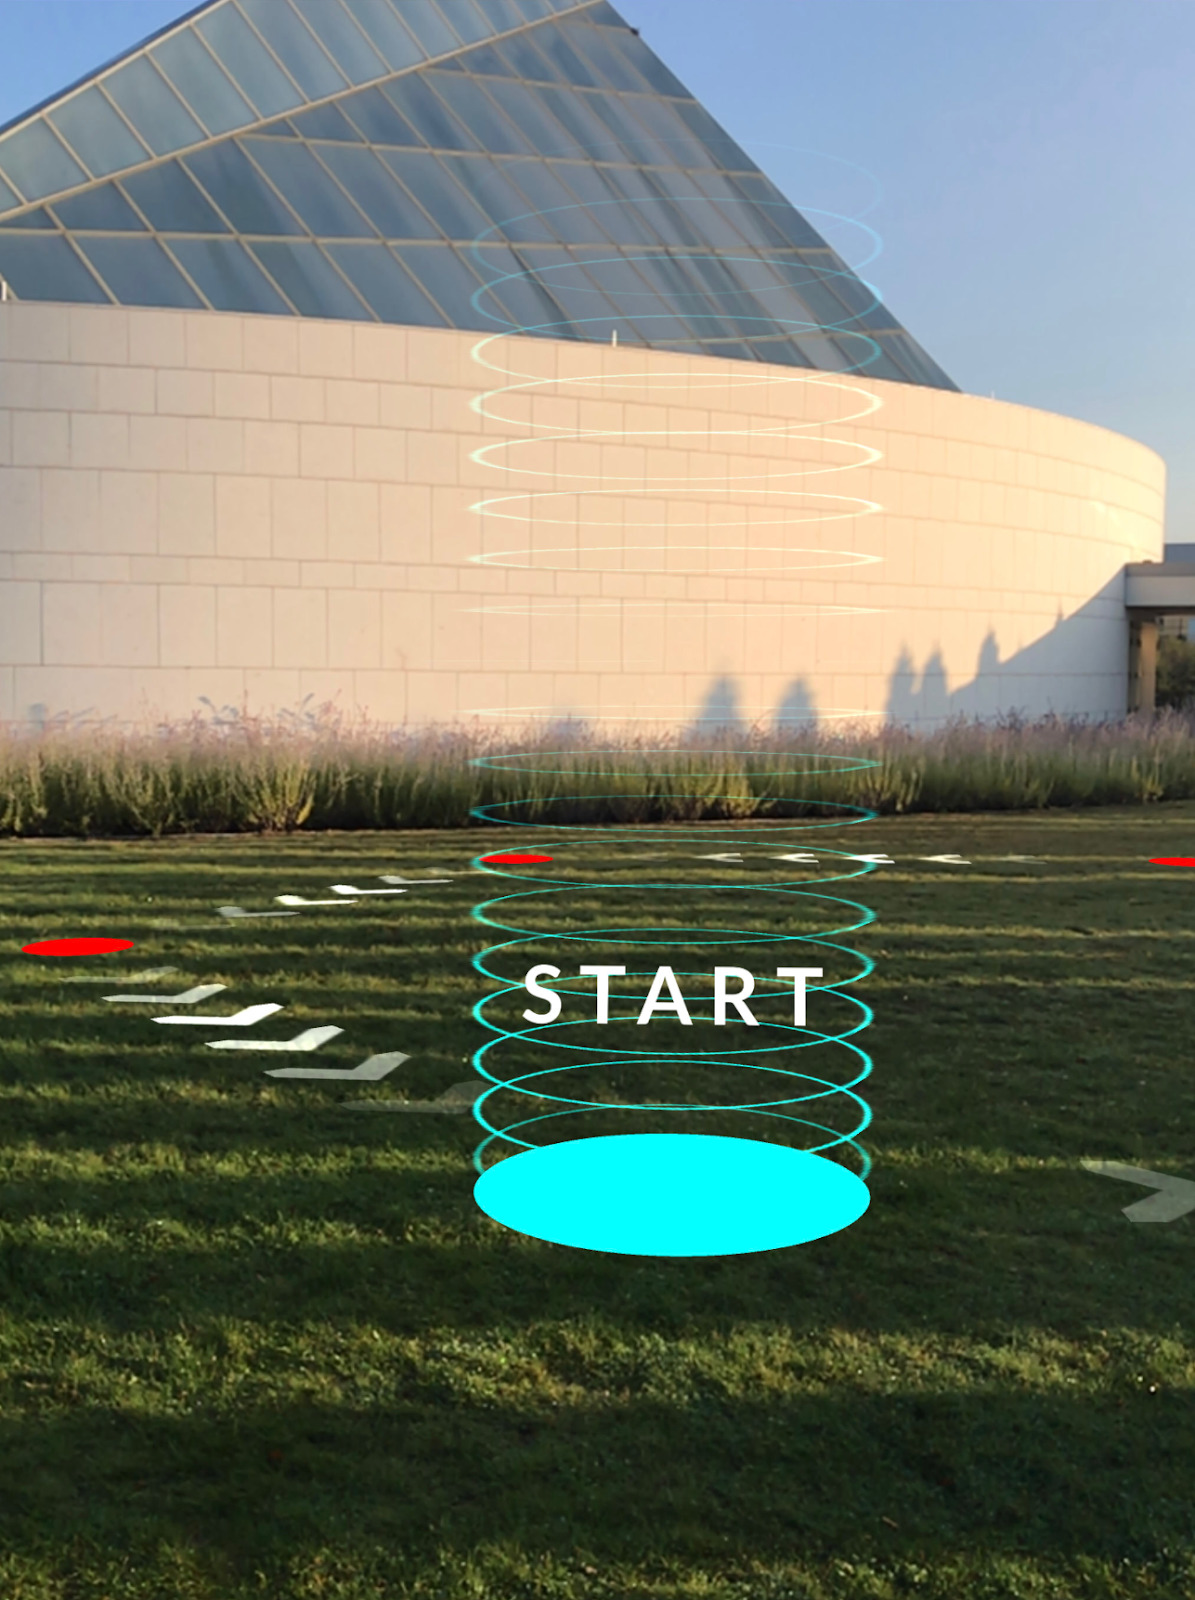
\includegraphics[scale=0.1]{arrunner}
      \caption{Imagen que muestra el juego AR Runner.\protect\footnotemark}
      \label{figura-ar-runner}
    \end{figure}

    \footnotetext{ \url{https://itunes.apple.com/us/app/ar-runner/id1275938861?mt=8}, Semidome Inc.}
  \end{itemize}

  \item \textbf{Astronomía}: Consisten en mostrarnos las constelaciones y elementos del universo basado en nuestra geolocalización, y estos se muestran sobre lo que la cámara recibe, es decir si quieres ver las constelaciones por la noche apuntas con la cámara y te indica donde estas están y te las muestra facilitando su visualización y localización.

  \begin{itemize}
    \item \textbf{Night Sky}: Esta aplicación consiste en visualizar las constelaciones, satélites y más elementos del universo, mostrandote donde se encuentran cada uno de los elementos para facilitar al usuario su visualización. La realidad aumentada aporta una mejor experiencia de usuario, al facilitar el proceso de encontrar donde se sitúan estos elementos, ya que al mostrar sobre lo que percibe la cámara es más fácil para el usuario localizarlo.

    \begin{figure}[h]
      \centering
      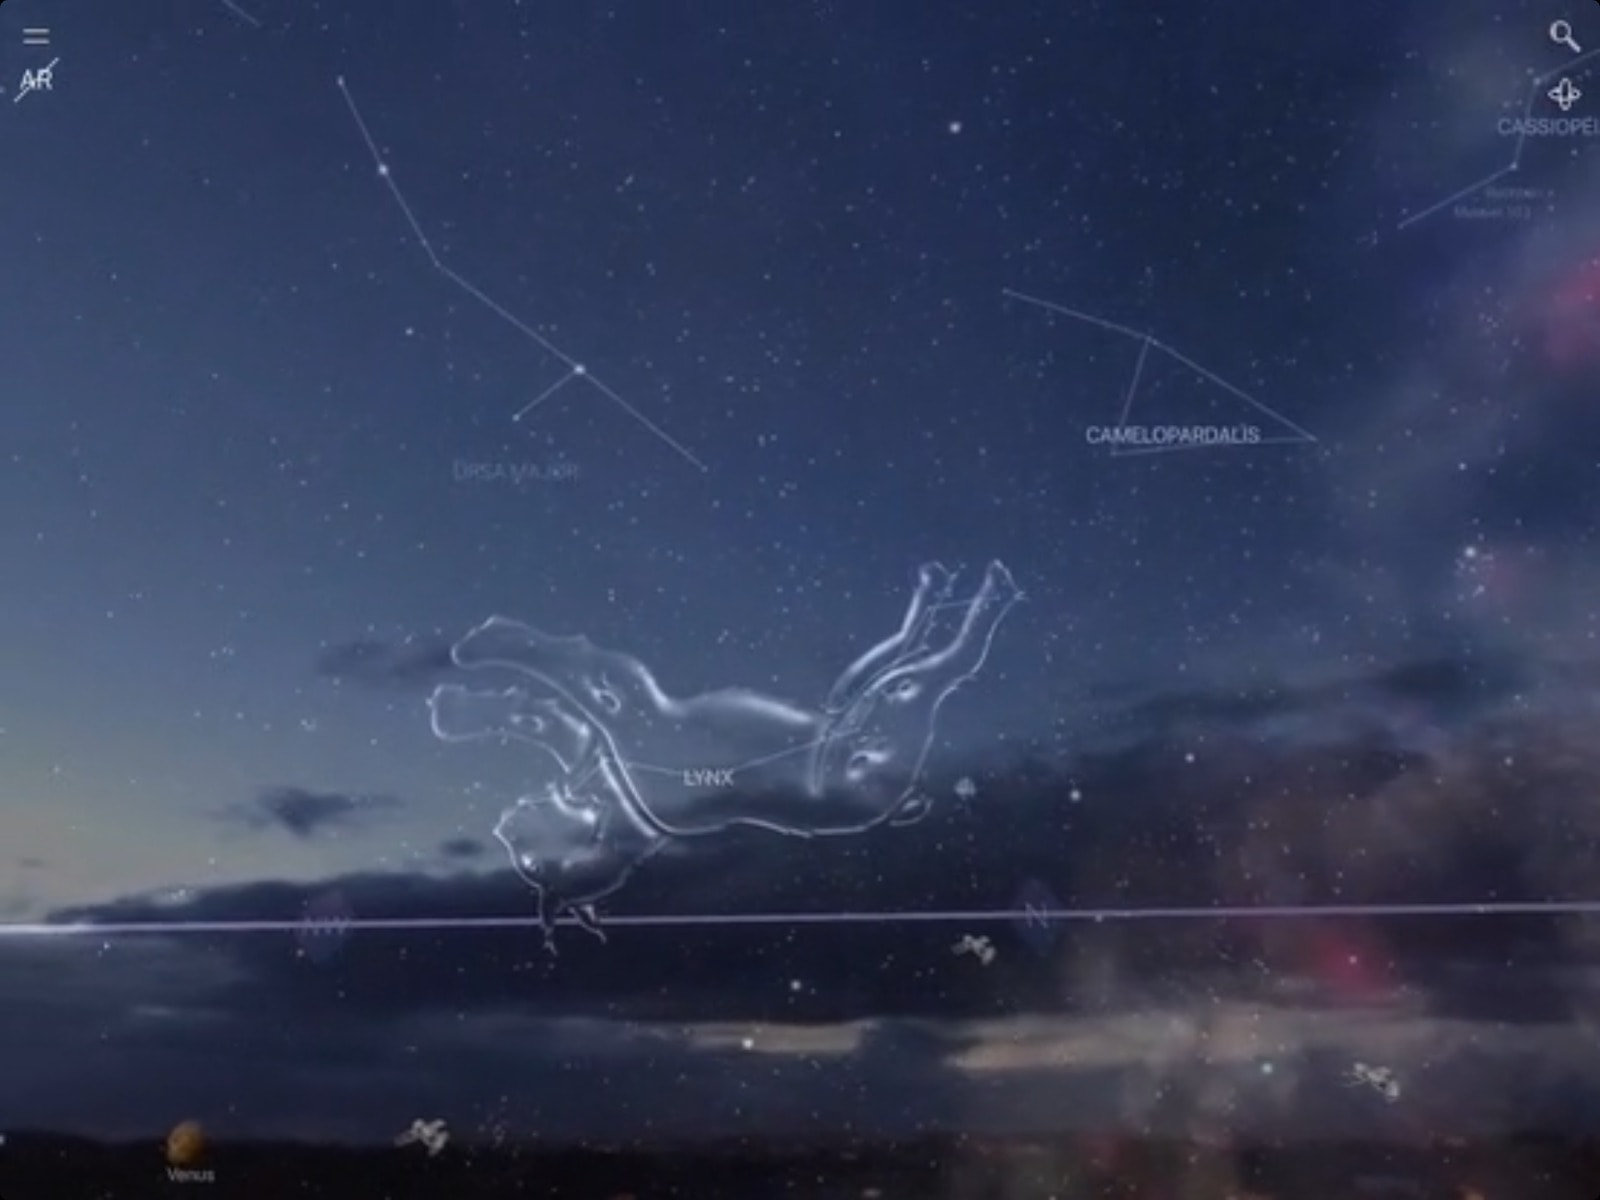
\includegraphics[scale=0.12]{nightsky}
      \caption{Imagen que muestra la aplicación Night Sky.\protect\footnotemark}
      \label{figura-night-sky}
    \end{figure}

    \footnotetext{ \url{https://itunes.apple.com/es/app/night-sky/id475772902?mt=8}, iCandi Apps}
  \end{itemize}

  \item \textbf{Utilidades}: Permiten al usuario llevar a cabo varias tareas que antes eran más difíciles de realizar o para las que necesitabas un dispositivo especial para realizarlas, y que ahora se pueden hacer solamente con tu un smartphone.

  \begin{itemize}
    \item \textbf{AR MeasureKit}: Esta aplicación permite realizar mediciones en el mundo real utilizando solo la camara. La realidad aumentada permite en este caso realizar una tarea que antes era imposible si no disponías de algún dispositivo de medida.

    \begin{figure}[h]
      \centering
      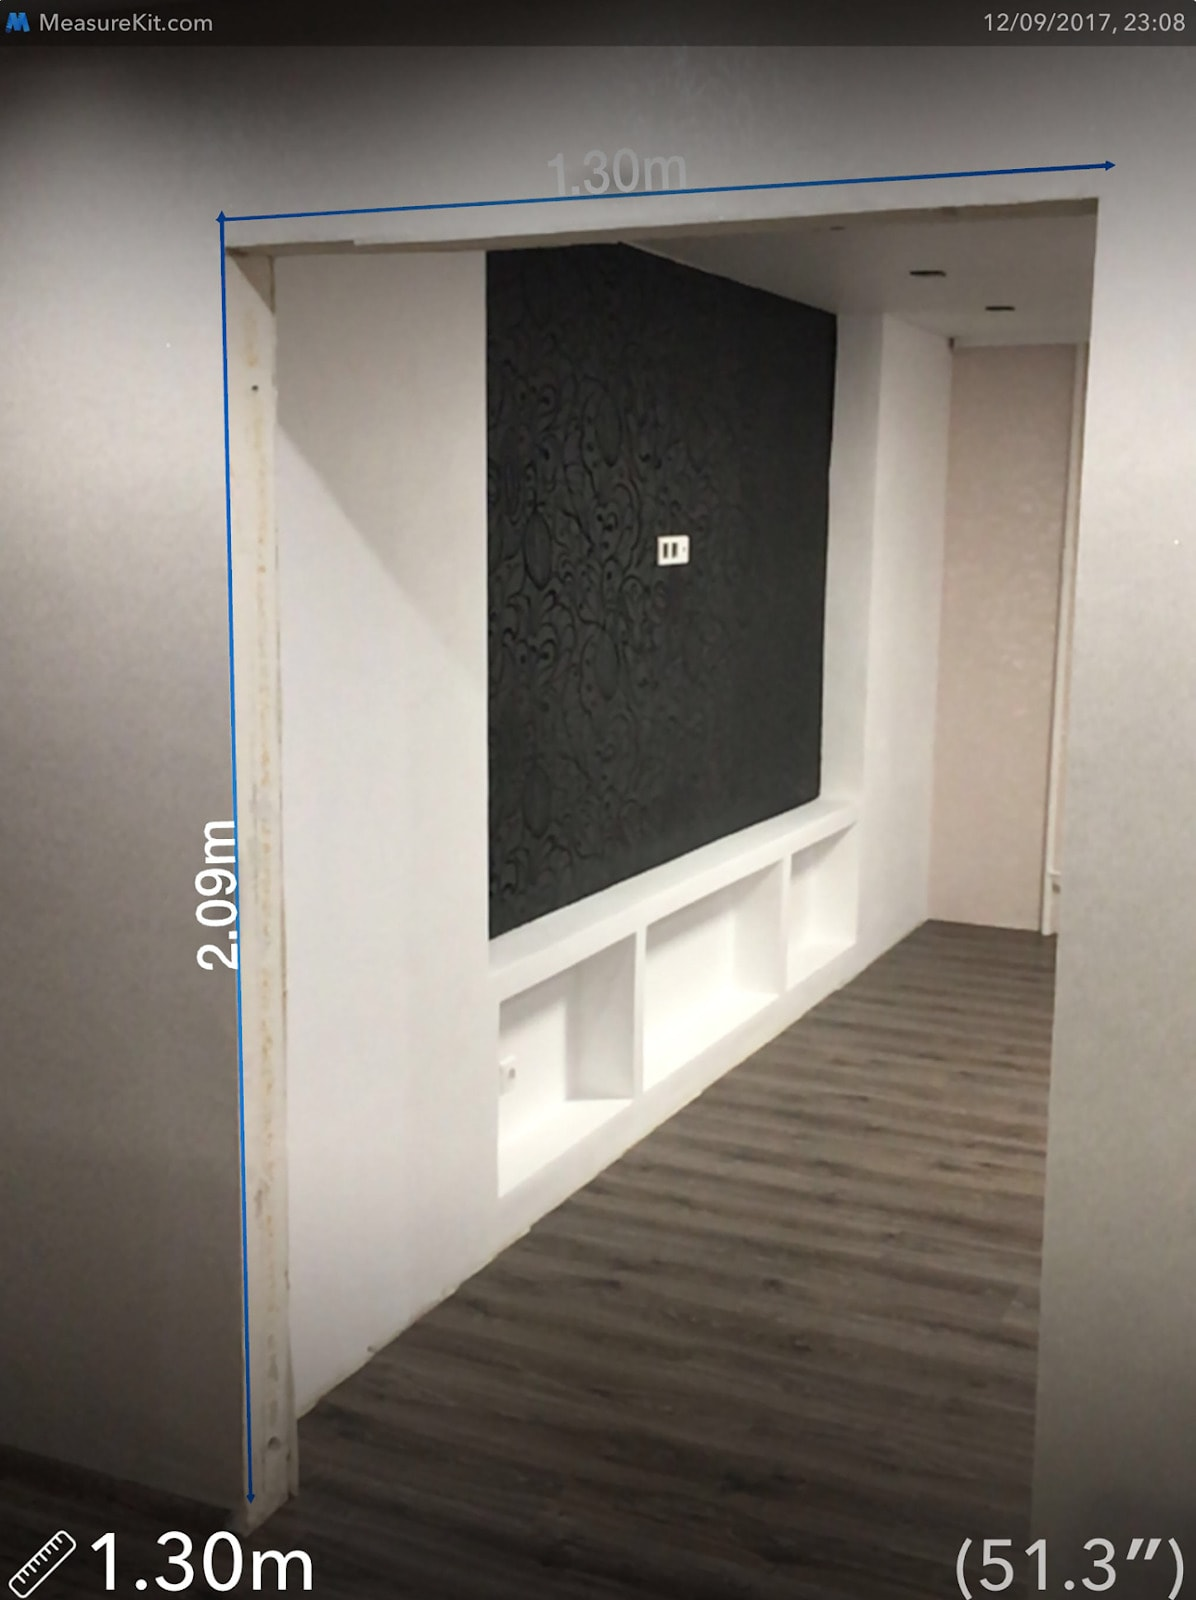
\includegraphics[scale=0.12]{armeasurekit}
      \caption{Imagen que muestra la aplicación AR MeasureKit.\protect\footnotemark}
      \label{figura-ar-measurekit}
    \end{figure}

    \footnotetext{ \url{https://itunes.apple.com/es/app/ar-measurekit/id1258270451?mt=8}, Rinat Khanov}
  \end{itemize}

  \item \textbf{Entretenimiento}: La funcionalidad principal es generar el entretenimiento del usuario o la creación de contenido situando elementos virtuales a el entorno físico y después fotografiando o grabando.

  \begin{itemize}
    \item \textbf{Monster Park}: Esta aplicación te permite colocar diferentes dinosaurios en tu propia habitación permitiendote hacer fotos o videos con ellos en la escena. La realidad aumentada permite que fotos con elementos inusuales, como puede ser un dinosaurio, se puedan realizar sin necesidad de photoshop y muchas horas de trabajo, y consiguiendo un mejor resultado.

    \begin{figure}[h]
      \centering
      
\includegraphics[scale=0.12]{monsterpark}
      \caption{Imagen que muestra la aplicación Monster Park.\protect\footnotemark}
      \label{figura-monster-park}
    \end{figure}

    \footnotetext{ \url{https://itunes.apple.com/es/app/monster-park-mundo-dinosaurio/id1259767702?mt=8}, Vito Technology Inc.}
  \end{itemize}

  \item \textbf{Educación}: Son aplicaciones que tienen un propósito educativo o de compartir conocimientos.

  \begin{itemize}
    \item \textbf{Insight heart}: Es una aplicación que te permite ver en 3D el corazón y sistema circulatorio. La realidad aumentada permite una forma mucho más sencilla, útil e intuitiva de entender el cuerpo humano, ya que al poder explorarlo moviéndote alrededor de este es mucho más natural y puedes ver todo mejor.

    \begin{figure}[h]
      \centering
      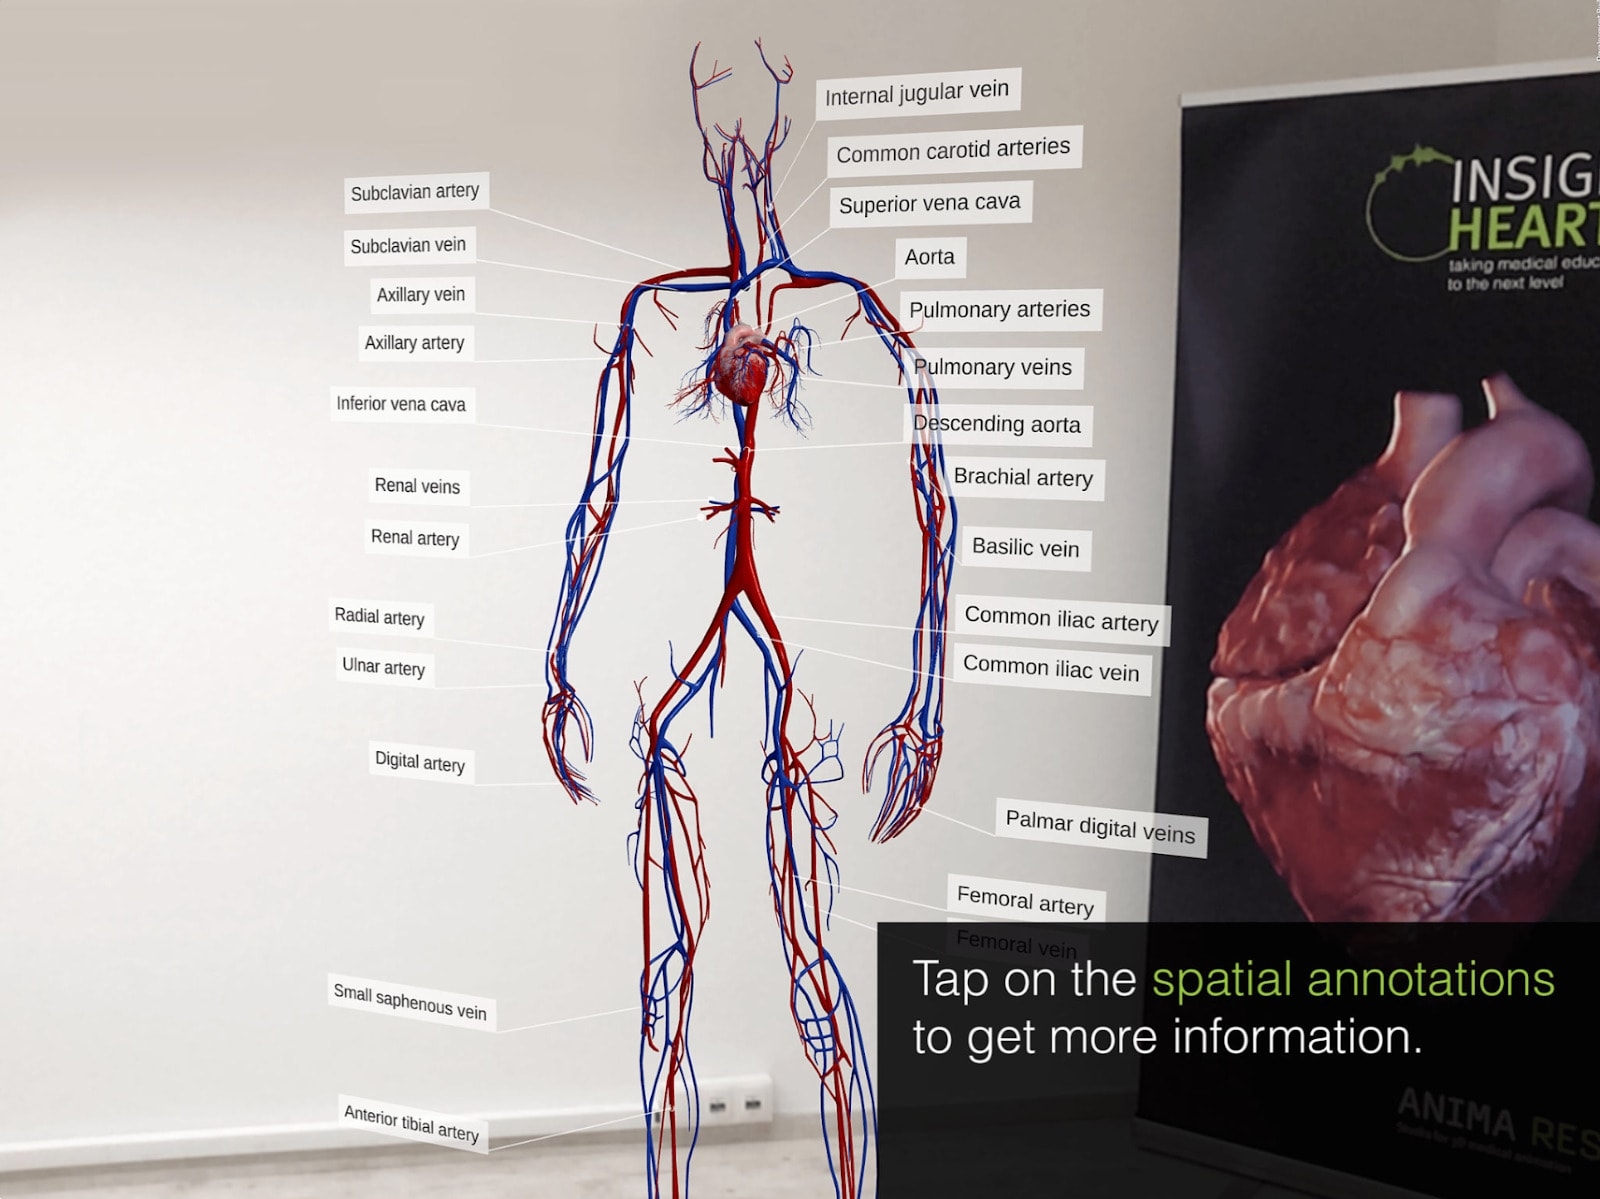
\includegraphics[scale=0.12]{insightheart}
      \caption{Imagen que muestra la aplicación Insight Heart.\protect\footnotemark}
      \label{figura-insight-heart}
    \end{figure}

    \footnotetext{ \url{https://itunes.apple.com/us/app/insight-heart/id1280845473?mt=8}, ANIMA RES}
  \end{itemize}
\end{itemize}

%%%%%%%%%%%%%%%%%%%%%%%%%%%%%%%%%%%%%%%%%%% ESTUDIO DE MERCADO APPS AR %%%%%%%%%%%%%%%%%%%%%%%%%%%%%%%%%%%%%%%%%%%%%%%%%

\section{Estudio de mercado sobre juegos de mesa que hacen uso de realidad aumentada}

Este estudio de mercado explora la forma en la que se aprovecha la realidad aumentada en los juegos de mesa en la actualidad:

\begin{itemize}
  \item \textbf{Chess+ AR}: Sobre una superficie plana sitúa un tablero virtual de ajedrez, en el que se puede jugar una partida moviendo las fichas, llevando a cabo la interacción con el juego de manera virtual, es decir, a través de la pantalla.

  \begin{figure}[h]
    \centering
    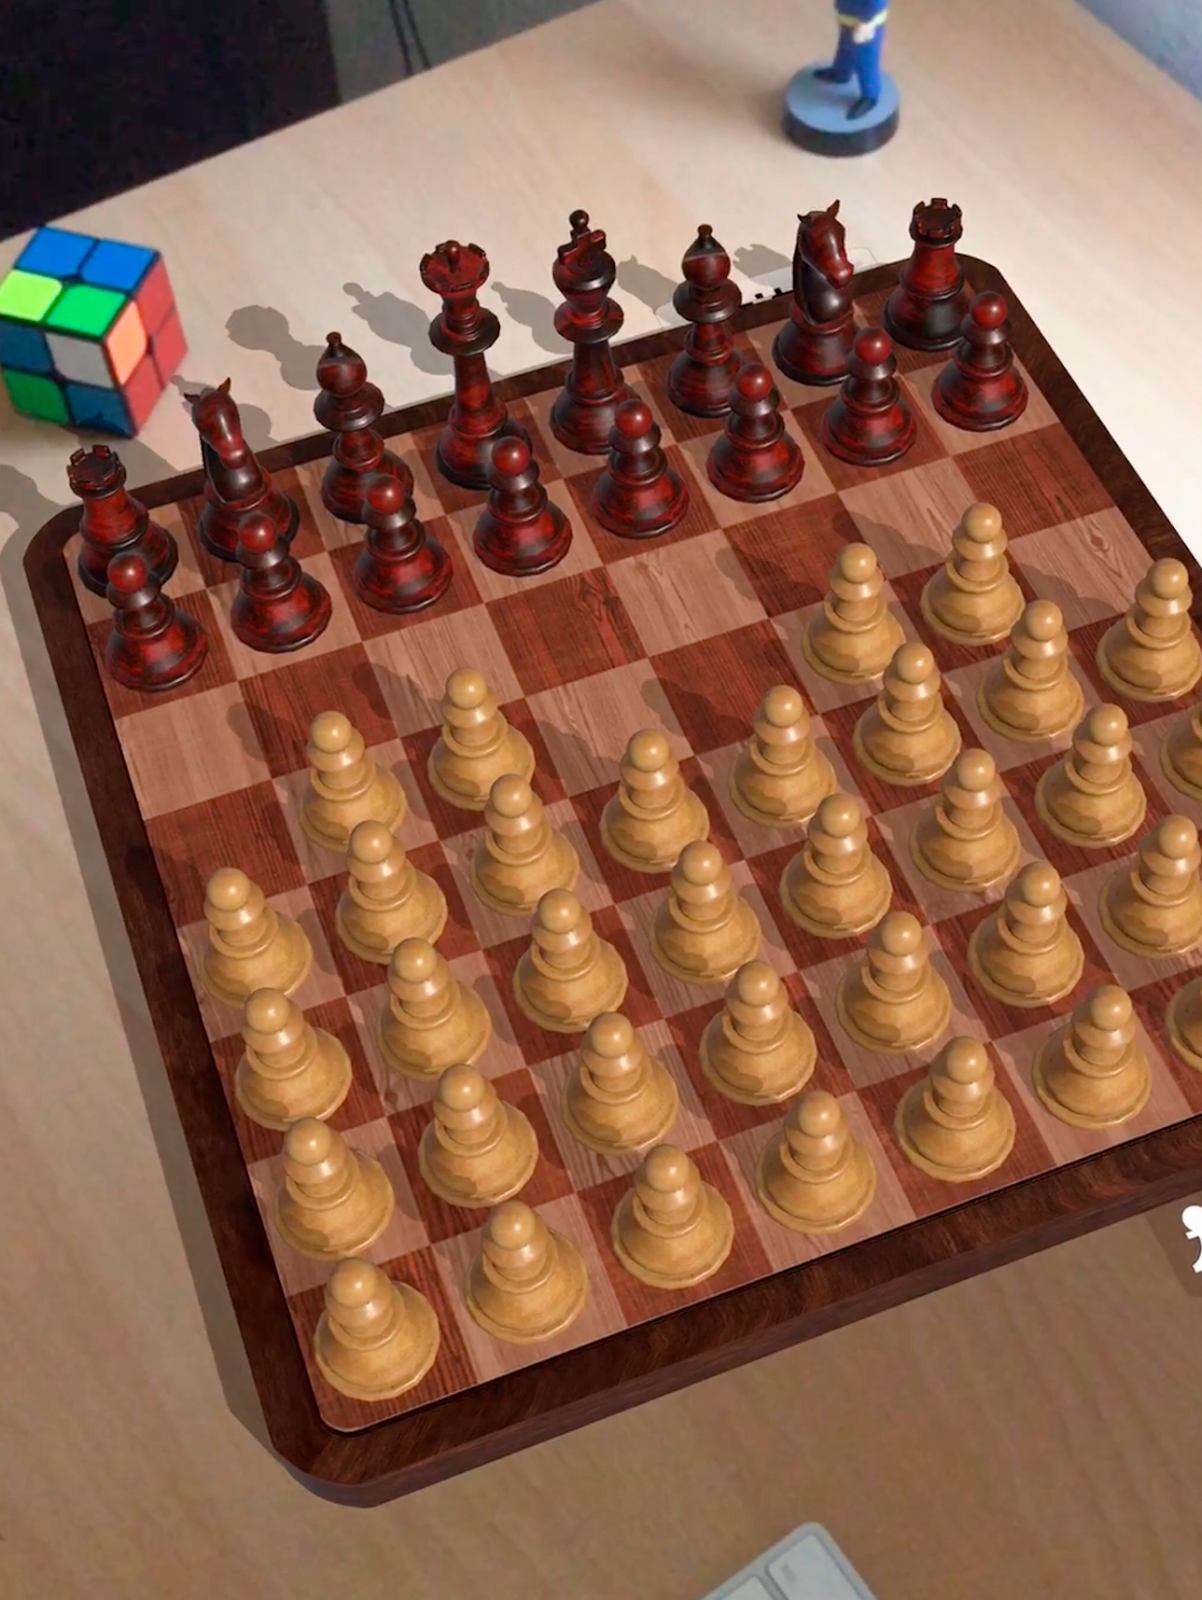
\includegraphics[scale=0.1]{chess}
    \caption{Imagen que muestra el juego Chess+ AR.\protect\footnotemark}
    \label{figura-siege-breakers}
  \end{figure}

  \footnotetext{ \url{https://itunes.apple.com/us/app/chess-ar/id1273831380?mt=8}, Jorge Moreno Aguilera}

  \newpage

  \item \textbf{AR Sea Wars}: Sobre una superficie plana se sitúa un tablero virtual, en este tu puedes colocar tus barcos y jugar para hundir los del adversario interactuando con la pantalla de forma virtual.

  \begin{figure}[h]
    \centering
    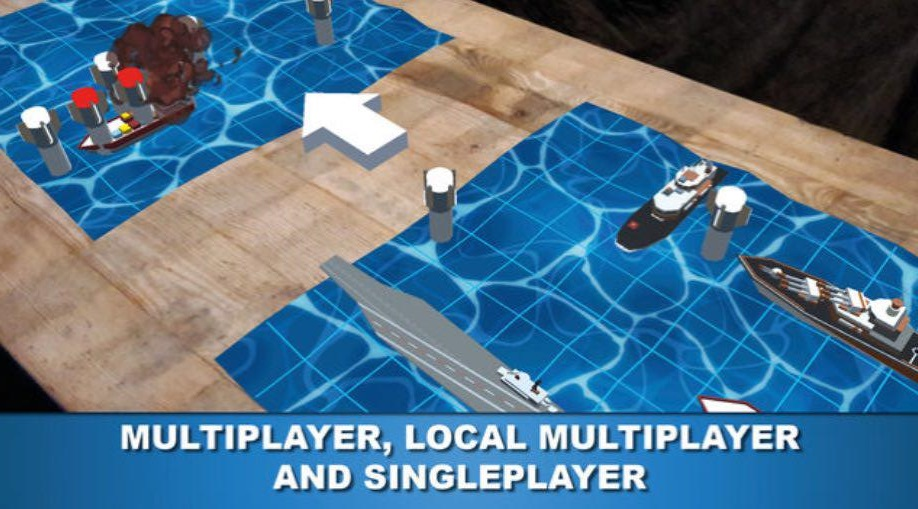
\includegraphics[scale=0.3]{sea-wars}
    \caption{Imagen que muestra el juego AR Sea Wars.\protect\footnotemark}
    \label{figura-sea-wars}
  \end{figure}

  \footnotetext{ \url{https://itunes.apple.com/us/app/ar-sea-wars/id1334666859?mt=8}, Dutch Rose Media}

  \item \textbf{AR Tic Tac Toe Multiplayer}: Sobre una superficie plana sitúa un tablero del juego “tres en raya”, y mediante la pantalla eliges donde poner el circulo o la cruz, por tanto, la interacción con el juego se hace completamente de manera virtual.

  \begin{figure}[h]
    \centering
    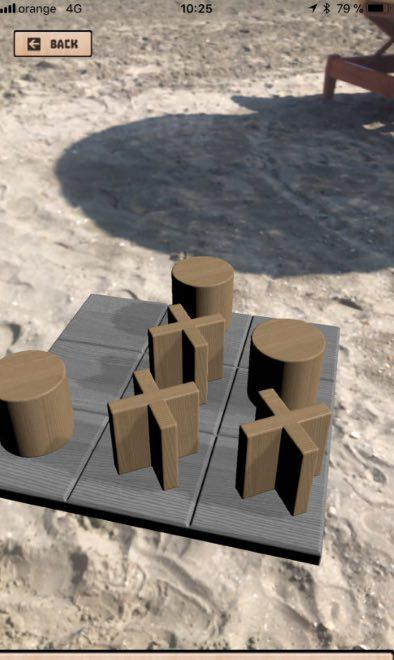
\includegraphics[scale=0.3]{tic-tac-toe}
    \caption{Imagen que muestra el juego AR Tic Tac Toe Multiplayer.\protect\footnotemark}
    \label{figura-tic-tac-toe}
  \end{figure}

  \footnotetext{ \url{https://itunes.apple.com/es/app/ar-tic-tac-toe-multiplayer/id1266613567?mt=8}, Code House Software SRL}

  \newpage

  \item \textbf{Roar! AR Boardgame hybrid game}: Permite al detectar el tablero de juego, establecer los elementos virtuales que servirán para el juego sobre este, convirtiendo parte de esa interacción en física y dando así un toque de realismo al juego.

  \begin{figure}[h]
    \centering
    
\includegraphics[scale=0.2]{roar-ar}
    \caption{Imagen que muestra el juego Roar! AR Boardgame hybrid game.\protect\footnotemark}
    \label{figura-roar-ar}
  \end{figure}

  \footnotetext{ \url{https://play.google.com/store/apps/details?id=com.TreflSA.Roar}, Trefl}

  \item \textbf{Augmented Reality Chess}: Permite al detectar marcadores establecer la pieza correspondiente a dicho marcador, y por tanto, permite jugar al juego mediante una interacción física, a partir del tablero y las fichas. Añadiendo así una sensación de realismo junto con la espectacularidad estética de la realidad aumentada.

  \begin{figure}[h]
    \centering
    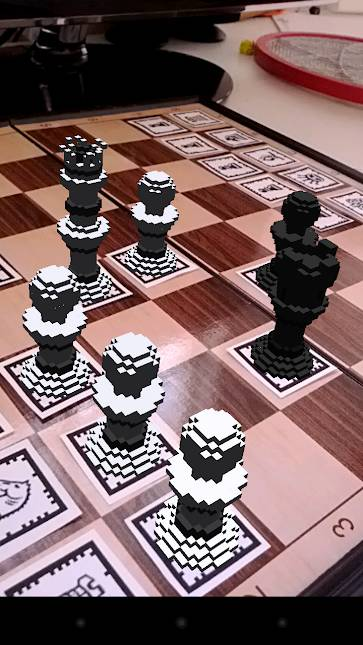
\includegraphics[scale=0.3]{augmented-reality-chess}
    \caption{Imagen que muestra el juego Augmented Reality Chess.\protect\footnotemark}
    \label{figura-augmented-reality-chess}
  \end{figure}

  \footnotetext{ \url{https://play.google.com/store/apps/details?id=com.contralabs.game.archess}, Contra Labs Oficial}

\end{itemize}

%%%%%%%%%%%%%%%%%%%%%%%%%%%%%%%%%%%%%%%%%%%%%%%%%%%%%%%%% CONCLUSIONES %%%%%%%%%%%%%%%%%%%%%%%%%%%%%%%%%%%%%%%%%%%%%%%%%%%%%%%%%
\section{Conclusiones}
Una vez realizado el estudio del arte, se ha llegado a las siguientes conlusiones:
\begin{itemize}
  \item La realidad aumentada es una tecnología que supondrá parte importante de las aplicaciones móviles en el futuro, ya que a pesar de estar empezando, ya se encuentra ciertamente avanzada para comenzar a ser utilizada, y el número de aplicaciones que esta ofrece es muy grande, abarcando desde el puro entretenimiento hasta el uso médico. El uso de esta tecnología en un juego de mesa es innovador y puede aportar una experiencia que mejore la de los juegos físicos y videojuegos tradicionales, combinando el mundo real y el virtual, en el punto exacto en el que se mantiene el realismo de un juego físico, y se aprovecha la espectacularidad visual de la realidad aumentada.

  \item El SDK ARCore es una apuesta segura para el desarrollo de aplicaciones que utilicen realidad aumentada en dispositivos móviles, dado que Google esta apostando fuertemente por esta tecnología. ARCore acaba prácticamente de nacer, y le queda mucho por mejorar, por lo que veremos muchos avances en los próximos meses y años, ofrecerá nuevas características que hasta ahora son probablemente inimaginables para la realidad aumentada en un dispositivo móvil de masas, todo esto hace que sea un valor seguro aprender como funciona este SDK y ser capaz de desarrollar aplicaciones móviles con él.

  \item Como se puede observar en el estudio realizado sobre aplicaciones que utilizan realidad aumentada, la mayoría de aplicaciones y juegos que utilizan realidad aumentada se basan en poner elementos virtuales en el mundo real, ya sea asociados a una imagen o en una superficie plana, pero sin realizar una combinación de lo real y virtual, por tanto, se puede observar la necesidad de juegos con realidad aumentada que utilicen elementos físicos para que no sea una experiencia puramente virtual, si no que se aprovechen los elementos virtuales para mejorar la realidad, de forma que se complementen.

  \item Por otro lado, en el estudio sobre juegos de mesa que utilizan realidad aumentada, se puede observar que la mayoría de estos juegos actualmente se basan en establecer todos los elementos sobre una superficie plana, sin embargo, solo unos pocos hacen uso de elementos físicos, lo que indica que hay un gran hueco para juegos que juntan componentes físicos con realidad aumentada, lo que permite que manteniendo una experiencia realista gracias a los elementos físicos, se pueda disfrutar de la espectacularidad de la realidad aumentada.

\end{itemize}

Estas conclusiones nos han llevado a establecer unos requisitos para el proyecto, con respecto al uso de la realidad aumentada:

\begin{itemize}
  \item El juego deberá contener los elementos enlazados a un tablero físico, de forma que mantenga un cierto realismo.

  \item Se permitirá realizar ciertas acciones utilizando cartas, para así añadir una forma de interacción física en el juego, obteniendo el realismo que se quiere alcanzar.

  \item Habrá que mantener un balance entre elementos físicos y virtuales, para que a la vez que aprovecha el potencial de la realidad aumentada, siga manteniendo el realismo de un juego físico.

  \item Deberá ser posible interactuar con algunos de los elementos 3D asociados al juego, para que no sea simplemente situarlos en un sitio y manejar el juego como si fuera un videojuego tradicional, si no aprovechar las posibilidades de la realidad aumentada, y trasladar toda la interacción posible con el juego a los elementos 3D.

\end{itemize}

\chapter{Proceso de desarrollo}
\label{ch:desarrollo}

\section{Metodologías de desarrollo ágil}

\section{Diseño centrado en el usuario}

\section{Plan de entregas}

\section{Bocetos}
Se han llevado a cabo pruebas sobre los bocetos que se encuentran en la sección \ref{bocetos} del Anexo, dichas pruebas incluyen pruebas heurísticas realizadas por el desarrollador y pruebas se usabilidad con usuarios reales.

\subsection{Pruebas heurísticas}
\begin{itemize}

  \item \textbf{Principio 1: Visibilidad del estado del sistema.}\\
  La puntuación es de 7, el usuario está bien informado de lo que ocurre actualmente en el sistema, se muestra siempre que es necesario el botón “home” o el botón “atrás”, pero se puede mejorar, por ejemplo, indicando que se están escaneando imágenes mientras mueves el dispositivo sobre el tablero.

  \item \textbf{Principio 2: Correspondencia entre el sistema y el mundo real.}\\
  La puntuación es de 10, las opciones en los menús están ordenadas de forma lógica y el lenguaje que el juego utiliza es un lenguaje común al usuario del juego.

  \item \textbf{Principio 3: Control y libertad del usuario.}\\
  La puntuación es de 7, ya que en la mayoría de pantallas el usuario es libre de ir hacia adelante o hacia atrás, pero en instrucciones el usuario puede avanzar al juego pero no volver a la pantalla de inicio. Además, como se puede ver en la pantalla 6, para hacer apuntes, el botón de retroceso está en la zona derecha de la pantalla, pudiendo confundir esto al usuario, ya que es una función de retroceso no de avance.

  \item \textbf{Principio 4: Consistencia y estándares.}\\
  La puntuación es de 7, ya que es bastante consistente, pero en la pantalla que indica el ganador aparece el botón “home” como en otras pantallas, pero se muestra en una posición distinta, lo que resulta confuso al usuario habría que moverlo a la posición que ocupa siempre o utilizar otro botón.

  \item \textbf{Principio 5: Prevención de errores.}\\
  La puntuación es de 10, el diseño es bastante cuidadoso para la prevención de errores y el correcto tratamiento de estos.

  \item \textbf{Principio 6: Minimizar la carga de memoria del usuario.}\\
  La puntuación es de 10, el usuario no necesita recordar nada en ningún momento, todo se muestra de forma apropiada para que no suponga ninguna memorización al usuario.

  \item \textbf{Principio 7: Personalización y atajos.}
  La puntuación es de 10, la aplicación no dispone de personalización o atajos, pero no son necesarios en esta, por lo que no afecta a la experiencia de usuario.

  \item \textbf{Principio 8: Eficiencia de uso y rendimiento.}
  La puntuación es de 8, la aplicación está bien optimizada para que al usuario le resulte sencillo y rápido llevar a cabo cualquier tarea, pero si es cierto que algunos botones que se utilizan con mucha frecuencia no están en las posiciones óptimas.

  \item \textbf{Principio 9: Estética y diseño minimalista.}
  La puntuación es de 10, la información que se muestra en la aplicación es la necesaria para que el usuario pueda jugar con la mejor experiencia de usuario posible, no hay exceso o falta de información.

  \item \textbf{Principio 10: Ayuda al usuario a reconocer, diagnosticar y recuperarse de errores.}
  La puntuación es de 10, ya que no hay posibilidad de que ocurran errores en el juego.

  \item \textbf{Principio 11: Ayuda y documentación.}
  La puntuación es de 10, ya que antes de comenzar cada partida se muestra al usuario unas instrucciones de cómo funciona el juego.

  \item \textbf{Principio 12: Interacción física y ergonomía.}
  La puntuación es de 10, ya que los botones son fácilmente diferenciables y están en una posición cómoda para el usuario, teniendo en cuenta que al ser un juego utilizará las dos manos para usar el dispositivo móvil.

\end{itemize}

\subsection{Pruebas de usabilidad}
Las tablas que contienen la información obtenida en estas pruebas de usabilidad se encuentran en la sección \ref{tablas-usabilidad-bocetos} del Anexo.

\begin{itemize}
  \item \textbf{Usuario 1}

  \textbf{Pre Test}

  \begin{enumerate}
    \item Edad: 18
    \item Dispone de un dispositivo móvil: Sí
    \item Con qué frecuencia utiliza su dispositivo móvil: Varias veces al dia
    \item Con qué frecuencia juega a juegos de mesa: Varias veces al año
    \item Con qué frecuencia juega a juegos en su móvil: Varias veces a la semana
  \end{enumerate}

  \textbf{Test}: Los resultados del test de usabilidad sobre el Usuario 1 se encuentran en la Tabla \ref{tabla-bocetos-usuario1}


  \item \textbf{Usuario 2}

  \textbf{Pre Test}

  \begin{enumerate}
    \item Edad: 57
    \item Dispone de un dispositivo móvil: Sí
    \item Con qué frecuencia utiliza su dispositivo móvil: Varias veces al día
    \item Con qué frecuencia juega a juegos de mesa: Varias veces al año
    \item Con qué frecuencia juega a juegos en su móvil: Varias veces al día
  \end{enumerate}

  \textbf{Test}: Los resultados del test de usabilidad sobre el Usuario 2 se encuentran en la Tabla \ref{tabla-bocetos-usuario2}


  \item \textbf{Usuario 3}

  \textbf{Pre Test}

  \begin{enumerate}
    \item Edad: 26
    \item Dispone de un dispositivo móvil: Sí
    \item Con qué frecuencia utiliza su dispositivo móvil: Varias veces al dia
    \item Con qué frecuencia juega a juegos de mesa: Una vez al mes como máximo
    \item Con qué frecuencia juega a juegos en su móvil: Casi nunca
  \end{enumerate}

  \textbf{Test}: Los resultados del test de usabilidad sobre el Usuario 3 se encuentran en la Tabla \ref{tabla-bocetos-usuario3}

\subsection{Conclusiones}
Durante dichas pruebas hemos podido comprobar que la interfaz de la aplicación es amigable para los usuarios, que si bien han detectado algunos fallos, que serán solventados en el desarrollo del juego, por lo general han sabido realizar todas las tareas sin dificultad, desenvolviéndose con rapidez.\\

También se ha podido comprobar el interés de los usuarios por el funcionamiento de la realidad aumentada, resultándoles algo sorprendente y que sin duda tenían ganas de probar en las siguientes pruebas de usabilidad, lo que denota la esperada expectación de los usuarios de juegos y en general de dispositivos móviles sobre la realidad aumentada y las novedosas experiencias que esta aportará al ámbito de los dispositivos móviles.

\chapter{Conclusiones finales y futuro}
\label{ch:conclusiones}

\section{Conclusiones}

\section{Trabajo futuro}

\chapter{Anexos}
\label{ch:anexos}

\section{Bocetos} \label{bocetos}

Las siguientes imágenes recogen los bocetos realizados previos al desarrollo del juego.\\

Bocetos sobre la pantalla inicial y la pantalla de instrucciones:
\begin{figure}[h]
  \centering
  \subfigure{
  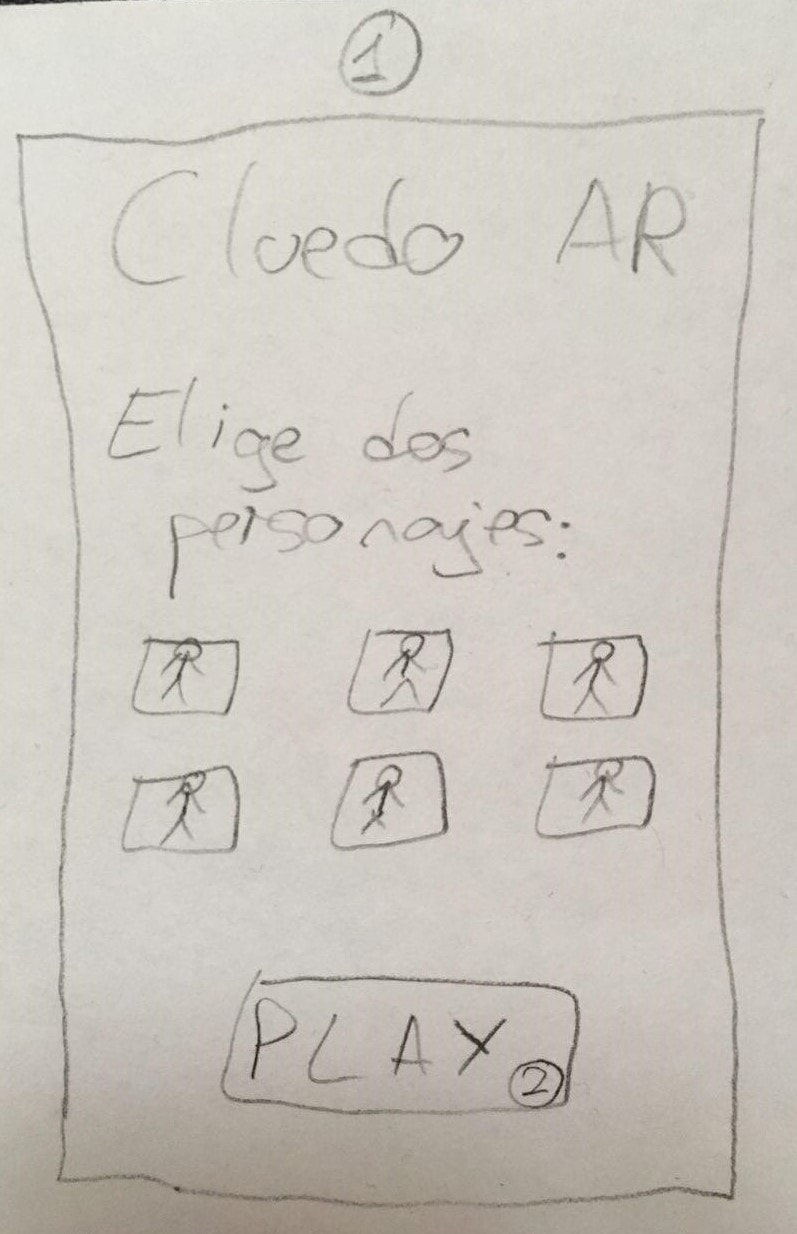
\includegraphics[height=3.5in]{b1.jpg}}
  \qquad
  \subfigure{
  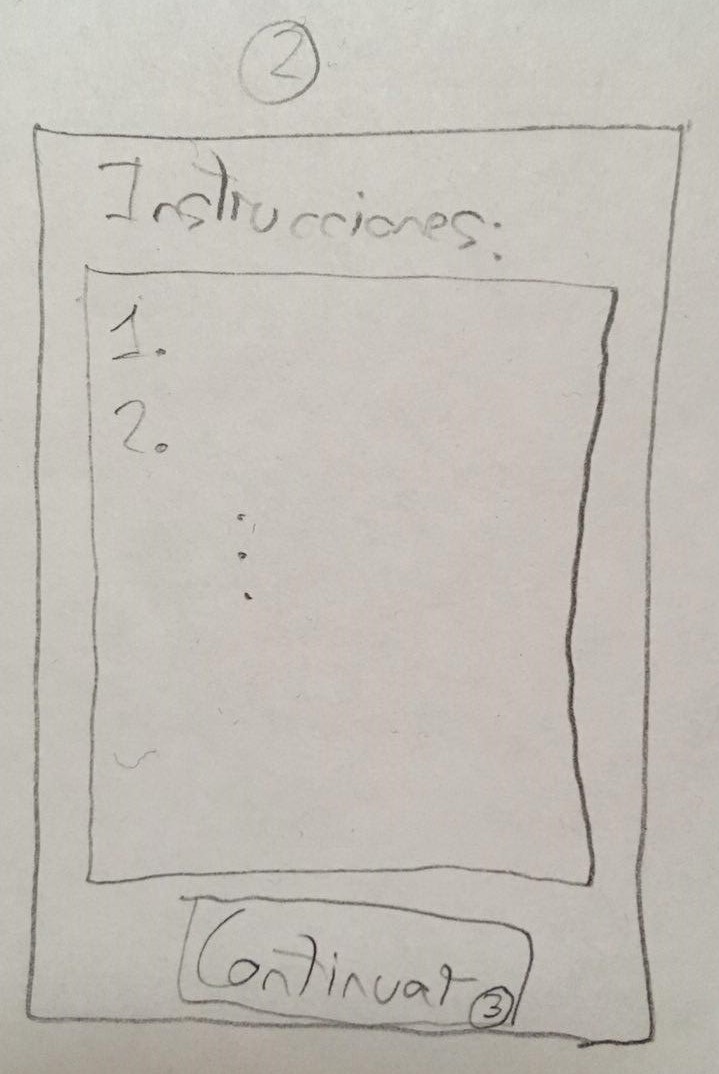
\includegraphics[height=3.5in]{b2.jpg}}
\end{figure}

\newpage

Bocetos sobre la pantalla de juego, con diferentes visualizaciones:

\begin{figure}[h]
  \subfigure{
  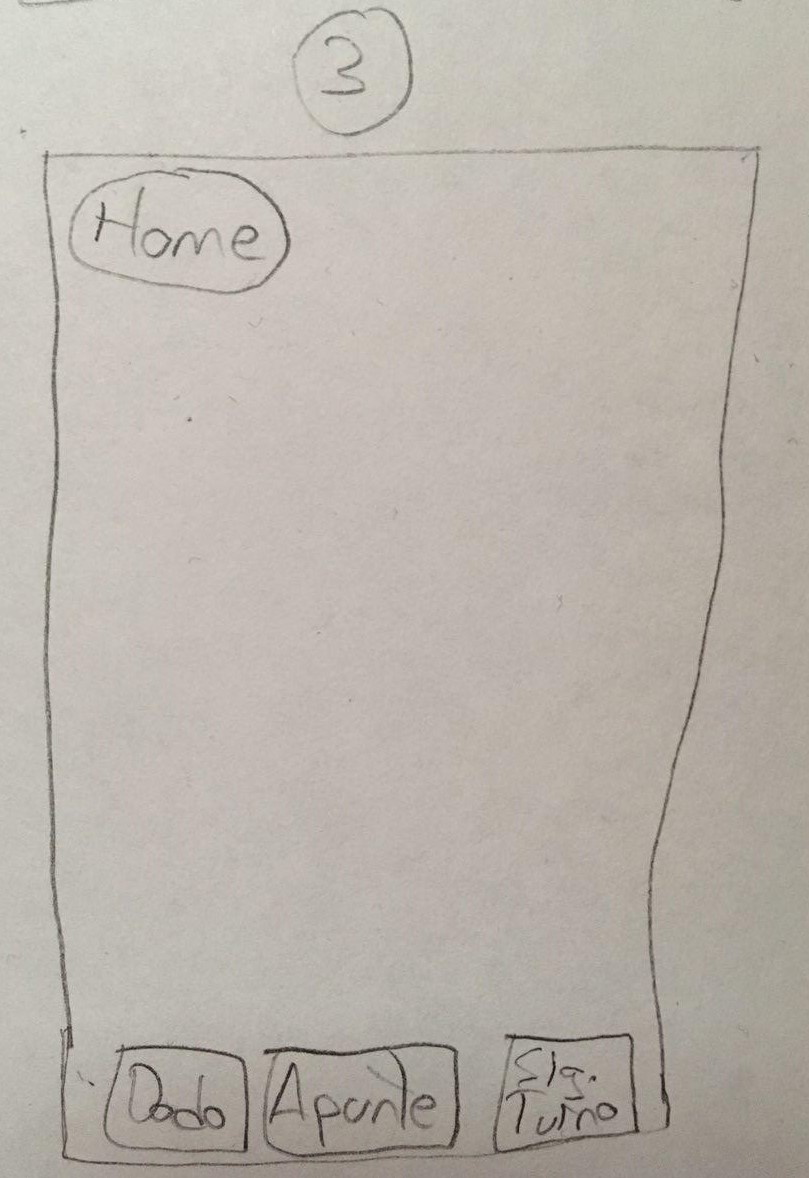
\includegraphics[height=3.05in]{b3.jpg}}
  \qquad
  \subfigure{
  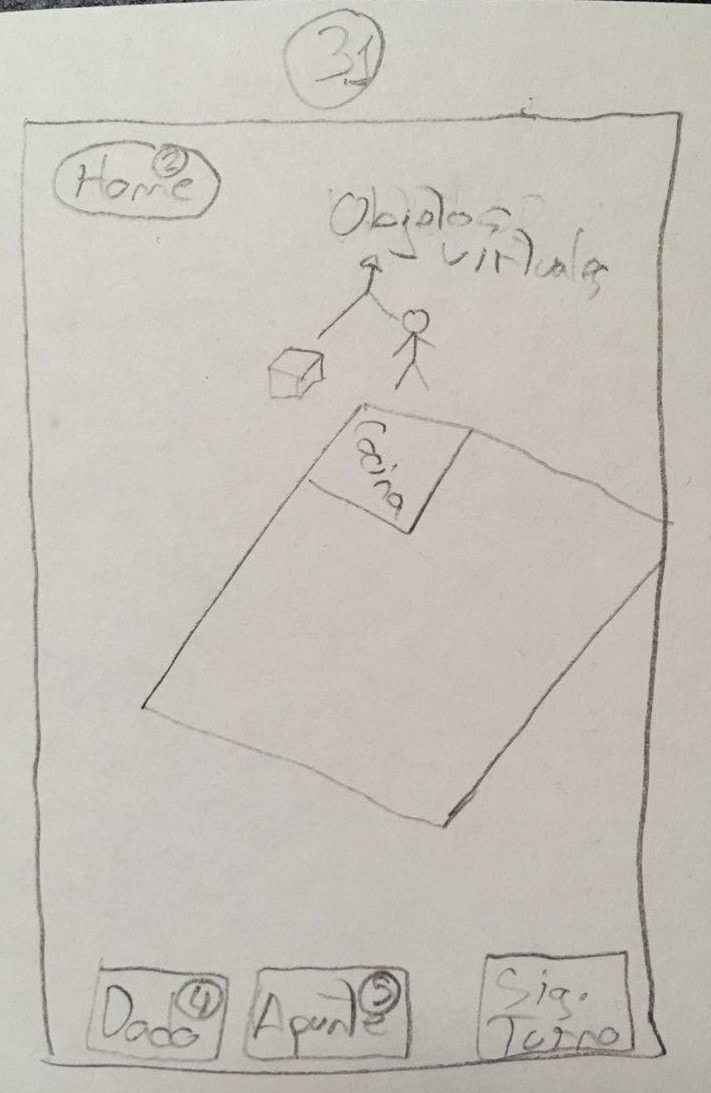
\includegraphics[height=3.1in]{b3-1.jpg}}
\end{figure}

Bocetos sobre la pantalla de juego, y la de selección de habitación:

\begin{figure}[h]
  \centering
  \subfigure{
  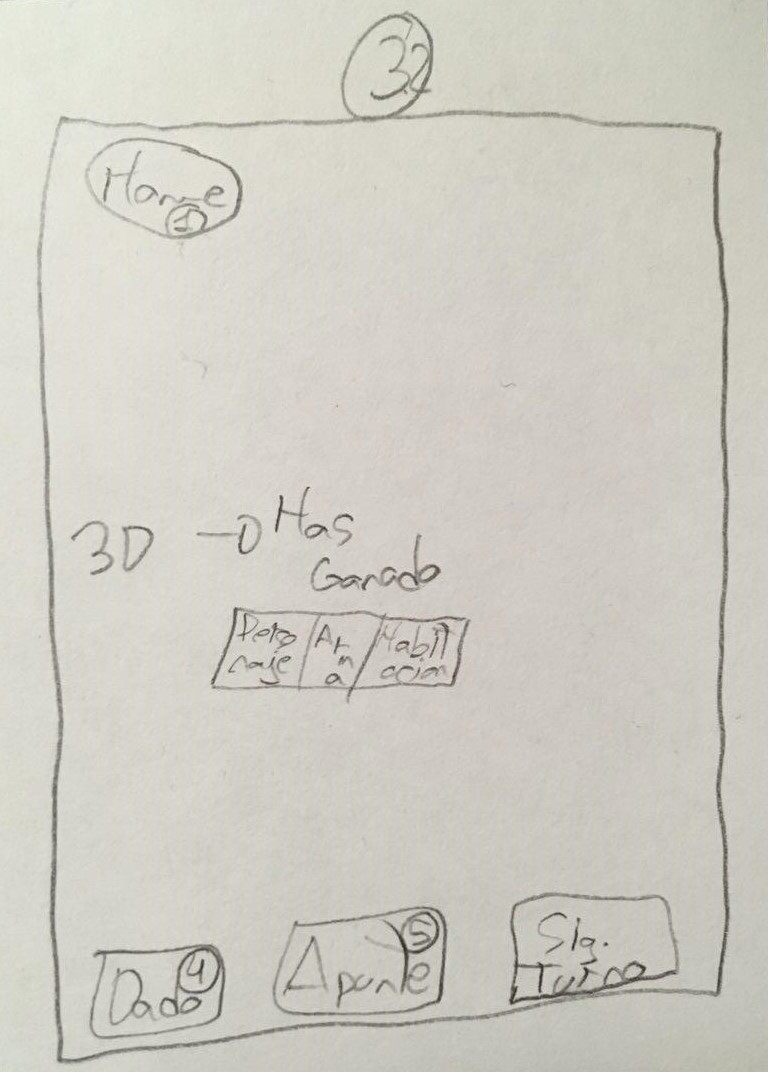
\includegraphics[height=2.95in]{b3-2.jpg}}
  \qquad
  \subfigure{
  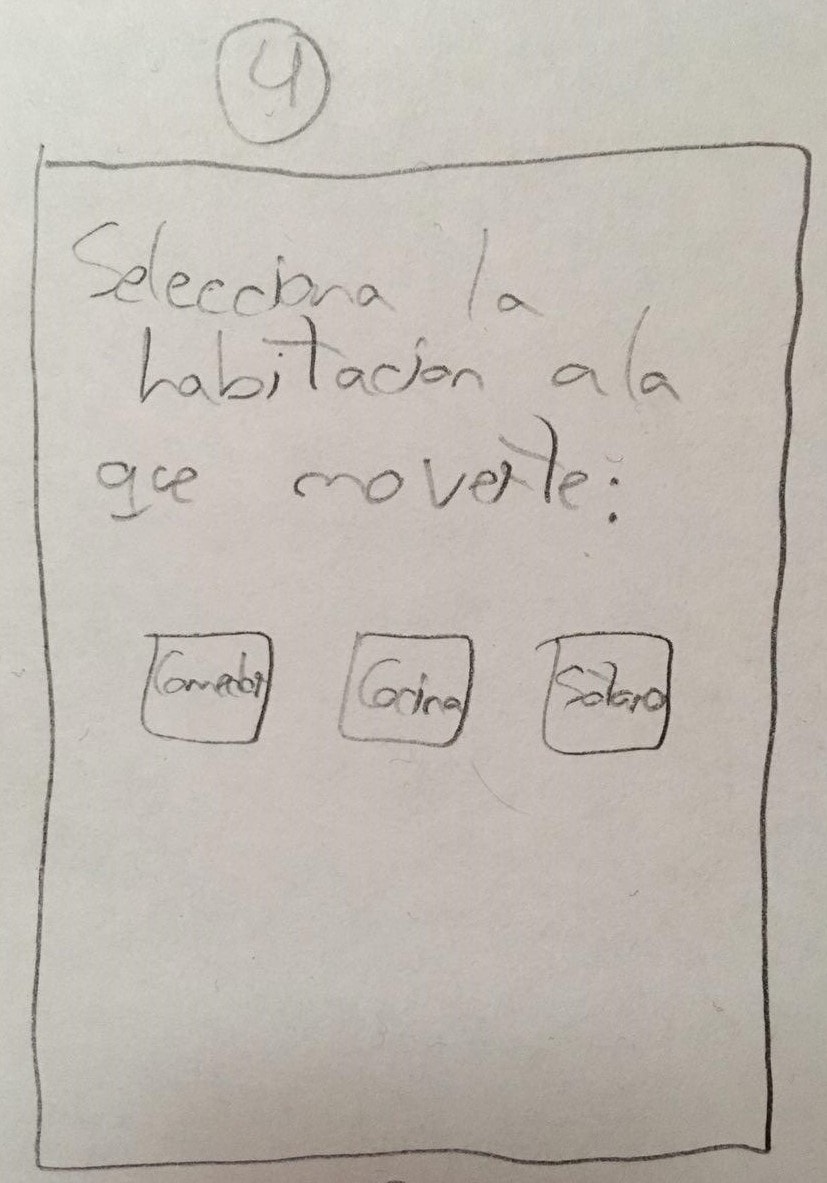
\includegraphics[height=2.95in]{b4.jpg}}
\end{figure}

\newpage

Bocetos sobre la pantalla de tomar apuntes y la pantalla cuando un jugador gana el juego:

\begin{figure}[h]
  \centering
  \subfigure{
  \includegraphics[height=3in]{b5.jpg}}
  \qquad
  \subfigure{
  \includegraphics[height=3in]{b6.jpg}}
\end{figure}


\section{Tablas de usabilidad para los bocetos} \label{tablas-usabilidad-bocetos}

\begin{table}
  \begin{center}
    \begin{tabular}{|p{2.5cm}|p{1.75cm}|p{1.25cm}|p{1.25cm}|p{2.75cm}|p{3.5cm}|}

      \hline
        \rowcolor{Gray} \textbf{Escenario de uso}
        & \textbf{Tarea}
        & \textbf{Éxito/ Fracaso}
        & \textbf{Tiempo}
        & \textbf{Dificultades encontradas}
        & \textbf{Comentarios}\\

      \hline
      El usuario se encuentra jugando una partida & Seleccionar ajustes iniciales
      & Éxito
      & 10 seg
      & Le cuesta seleccionar el personaje con el dedo
      & Hacer los botones de personaje mas grandes para facilitar a los usuarios este proceso\\

      \hline
      El usuario se encuentra jugando una partida
      & Comenzar el juego
      & Éxito
      & 5 seg
      & Ninguna
      &\\

      \hline
      El usuario se encuentra jugando una partida
      & Salir de las instrucciones
      & Éxito
      & 5 seg
      & Ninguna
      &\\

      \hline
      El usuario se encuentra jugando una partida
      & Escanear el tablero
      & Éxito
      & 10 seg
      & Ninguna
      &\\

      \hline
      El usuario se encuentra jugando una partida
      & Lanzar el dado
      & Éxito
      & 20 seg
      & Ninguna
      & Añadir imagen con el nombre de la habitación para facilitar a los usuarios este proceso\\

      \hline
      El usuario se encuentra jugando una partida
      & Hacer apunte
      & Éxito
      & 25 seg
      & Ninguna
      &\\

      \hline
      El usuario se encuentra jugando una partida
      & Escanear acusación
      & Éxito
      & 20 seg
      & Ninguna
      &\\

      \hline
      El usuario se encuentra jugando una partida
      & Pasar de turno
      & Éxito
      & 5 seg
      & Ninguna
      &\\

      \hline
      El usuario se encuentra jugando una partida
      & Volver a la pantalla inicial
      & Fracaso
      & 15 seg
      & No sabe donde seleccionar terminar partida
      & Cambiar el texto del botón home por Terminar partida\\

      \hline
      El usuario se encuentra jugando una partida
      & Finalizar después de ganar
      & Éxito
      & 5 seg
      & No sabe donde seleccionar para salir de esa pantalla
      & Cambiar el texto del botón home por Continuar\\

      \hline

    \end{tabular}

    \caption{Resultados usabilidad con Usuario 1.}
    \label{tabla-bocetos-usuario1}

  \end{center}
\end{table}


\begin{table}
  \begin{center}
    \begin{tabular}{|p{2.5cm}|p{1.75cm}|p{1.25cm}|p{1.25cm}|p{2.75cm}|p{3.5cm}|}

      \hline
        \rowcolor{Gray} \textbf{Escenario de uso}
        & \textbf{Tarea}
        & \textbf{Éxito/ Fracaso}
        & \textbf{Tiempo}
        & \textbf{Dificultades encontradas}
        & \textbf{Comentarios}\\

      \hline
      El usuario se encuentra jugando una partida
      & Seleccionar ajustes iniciales
      & Éxito
      & 5 seg
      & Ninguna
      &\\

      \hline
      El usuario se encuentra jugando una partida
      & Comenzar el juego
      & Éxito
      & 5 seg
      & Ninguna
      &\\

      \hline
      El usuario se encuentra jugando una partida
      & Salir de las instrucciones
      & Éxito
      & 5 seg
      & Ninguna
      &\\

      \hline
      El usuario se encuentra jugando una partida
      & Escanear el tablero
      & Éxito
      & 15 seg
      & Ninguna
      &\\

      \hline
      El usuario se encuentra jugando una partida
      & Lanzar el dado
      & Éxito
      & 10 seg
      & Ninguna
      & \\

      \hline
      El usuario se encuentra jugando una partida
      & Hacer apunte
      & Fracaso
      & 25 seg
      & No comprendía el funcionamiento de cómo realizar un apunte
      & Explicar en la pantalla de instrucciones inicial como se realiza un apunte\\

      \hline
      El usuario se encuentra jugando una partida
      & Escanear acusación
      & Éxito
      & 10 seg
      & Ninguna
      &\\

      \hline
      El usuario se encuentra jugando una partida
      & Pasar de turno
      & Éxito
      & 3 seg
      & Ninguna
      &\\

      \hline
      El usuario se encuentra jugando una partida
      & Volver a la pantalla inicial
      & Fracaso
      & 7 seg
      & No encontraba el botón de inicio
      & Cambiar el texto del botón a español y mas grande\\

      \hline
      El usuario se encuentra jugando una partida
      & Finalizar después de ganar
      & Éxito
      & 3 seg
      & No sabe que significa home, el botón es pequeño y poco accesible
      & Cambiar el texto del botón a español y mas grande\\

      \hline

    \end{tabular}

    \caption{Resultados usabilidad con Usuario 2.}
    \label{tabla-bocetos-usuario2}

  \end{center}
\end{table}


\begin{table}
  \begin{center}
    \begin{tabular}{|p{2.5cm}|p{1.75cm}|p{1.25cm}|p{1.25cm}|p{2.75cm}|p{3.5cm}|}

      \hline
        \rowcolor{Gray} \textbf{Escenario de uso}
        & \textbf{Tarea}
        & \textbf{Éxito/ Fracaso}
        & \textbf{Tiempo}
        & \textbf{Dificultades encontradas}
        & \textbf{Comentarios}\\

      \hline
      El usuario se encuentra jugando una partida
      & Seleccionar ajustes iniciales
      & Éxito
      & 5 seg
      & Ninguna
      & Activar el botón de play cuando haya seleccionado 2 personajes\\

      \hline
      El usuario se encuentra jugando una partida
      & Comenzar el juego
      & Éxito
      & 5 seg
      & Ninguna
      &\\

      \hline
      El usuario se encuentra jugando una partida
      & Salir de las instrucciones
      & Éxito
      & 5 seg
      & Ninguna
      &\\

      \hline
      El usuario se encuentra jugando una partida
      & Escanear el tablero
      & Éxito
      & 3 seg
      & Ninguna
      &\\

      \hline
      El usuario se encuentra jugando una partida
      & Lanzar el dado
      & Éxito
      & 15 seg
      & El botón de dado no era muy descriptivo y el usuario no sabia si ahí se lanzaba
      & Cambiar el texto del botón dado a Lanzar dado\\

      \hline
      El usuario se encuentra jugando una partida
      & Hacer apunte
      & Éxito
      & 20 seg
      & El botón usuario no entiende que pasa al pulsar el botón de apunte
      & Cambiar el texto del botón de apunte a Notas\\

      \hline
      El usuario se encuentra jugando una partida
      & Escanear acusación
      & Éxito
      & 10 seg
      & Ninguna
      &\\

      \hline
      El usuario se encuentra jugando una partida
      & Pasar de turno
      & Éxito
      & 3 seg
      & Ninguna
      &\\

      \hline
      El usuario se encuentra jugando una partida
      & Volver a la pantalla inicial
      & Éxito
      & 3 seg
      & Ninguna
      &\\

      \hline
      El usuario se encuentra jugando una partida
      & Finalizar después de ganar
      & Éxito
      & 3 seg
      & Ninguna
      & Camiar el texto a Continuar y cambiar su posición y tamaño\\

      \hline

    \end{tabular}

    \caption{Resultados usabilidad con Usuario 3.}
    \label{tabla-bocetos-usuario3}

  \end{center}
\end{table}

\end{itemize}


% Glosario de términos
\backmatter
\begingroup
	\setlength\parindent{0pt}
	\chapter{Glosario de términos}

\begin{description}
  
\end{description}

\endgroup

% Bibliografía
\newpage
\begin{thebibliography}{99}
	\addcontentsline{toc}{chapter}{Bibliografía}

\subsection*{Páginas web consultadas durante la realización del proyecto}

\bibitem{globalizacion} {\tt Globalización - Wikipedia}\\
\url{https://es.wikipedia.org/wiki/Globalizaci%C3%B3n}

\bibitem{globalreport} {\tt Globalization Report 2016 - Who benefits most from globalization?}\\
\url{https://www.bertelsmann-stiftung.de/fileadmin/files/BSt/Publikationen/GrauePublikationen/NW_Globalization_Report_2016.pdf}

\bibitem{internetusage} {\tt Wikipedia - Global Internet usage stats from the International Telecommunications Union}\\
\url{https://en.wikipedia.org/wiki/Global_Internet_usage#Internet_users}

\bibitem{ugremprende} {\tt UGR Emprendedora - Página principal}\\
\url{https://ugremprendedora.ugr.es/}

\bibitem{h2020} {\tt Horizon 2020 - Página principal}\\
\url{https://ec.europa.eu/programmes/horizon2020/}

\bibitem{agilereport} {\tt Top 10 Insights from the 11th Annual State of Agile Report}\\
\url{https://explore.versionone.com/state-of-agile/top-10-insights-from-the-11th-annual-state-of-agile-report-2}

\bibitem{health1} {\tt PubMed Central - Multidisciplinary in-hospital teams improve patient outcomes: A review}\\
\url{https://www.ncbi.nlm.nih.gov/pmc/articles/PMC4173201/}

\bibitem{health2} {\tt PubMed Central - Benefits of multidisciplinary teamwork in the management of breast cancer}\\
\url{https://www.ncbi.nlm.nih.gov/pmc/articles/PMC3929250/}

\bibitem{neuroped} {\tt Imagen original de NeuroPed - Enlace}\\
\url{http://www.neuroped.es/equipo-multidisciplinar/}

\bibitem{medialabugr} {\tt Medialab UGR - Página principal}\\
\url{http://medialab.ugr.es/}

\bibitem{linkuma} {\tt Link by UMA-ATech (Universidad de Málaga) - Página principal}\\
\url{http://www.link.uma.es/}

\bibitem{linkimage} {\tt Fotografía original de Geek and Tech Girls}\\
\url{https://geekandtechgirls.github.io/We-Create-Technology/}

\bibitem{linkedin} {\tt LinkedIn - Página principal}\\
\url{https://es.linkedin.com/}

\bibitem{kickstarter} {\tt Kickstarter - Página principal}\\
\url{https://www.kickstarter.com/}

\bibitem{responsivelink} {\tt Página de inicio de \textit{Responsive Web Design}}\\
\url{https://responsivedesign.is/}

\bibitem{contentwater} {\tt Imagen original de Wikimedia - Enlace}\\
\url{https://commons.wikimedia.org/wiki/File:Content_is_like_water.png}

\bibitem{framework} {\tt Framework - Wikipedia}\\
\url{https://es.wikipedia.org/wiki/Framework}

\bibitem{startup} {\tt Startup - Wikipedia}\\
\url{https://es.wikipedia.org/wiki/Empresa_emergente}

\bibitem{designthinkinglink} {\tt Design Thinking en Español - Página oficial}\\
\url{http://designthinking.es/inicio/index.php}

\subsection*{Libros consultados}

\bibitem{gangoffour}
Gamma, E., Helm, R., Johnson, R. and Vlissides, J. 1994. {\em Design Patterns. Elements of Reusable Object-Oriented Software}. Addison Wesley.

\bibitem{brandon}
M. Brandon, D. 2008. {\em Software Engineering for Modern Web Applications: Methodologies and Technologies}. Information Science Reference.

\bibitem{pressman}
Pressman, R. 1982. {\em Software Engineering - A Practitioner's Approach}. McGraw-Hill Higher Education.

\bibitem{pressmanweb}
Pressman, R. and Lowe, D. 2009. {\em Web Engineering - A Practitioner's Approach}. McGraw-Hill Higher Education.

\bibitem{headfirstpatterns}
Sierra, K., Freeman, E., Robson, E. and Bates, B. 2004. {\em Head First Dessign Patterns. A Brain-Friendly Guide}. O'Reilly.

\subsection*{Páginas de principales productos y programas usados}

\bibitem{bootstrap} {\tt Bootstrap Framework - Página principal}\\
\url{https://getbootstrap.com/}

\bibitem{laravel} {\tt Laravel - Página principal}\\
\url{https://laravel.com}

\bibitem{xampp} {\tt XAMPP - Página oficial}\\
\url{https://www.apachefriends.org/es/index.html}

\bibitem{slack} {\tt Slack - Página oficial}\\
\url{https://slack.com/}

\bibitem{googlecalendar} {\tt Google Calendar - Página oficial}\\
\url{https://www.google.com/calendar}

\bibitem{googledrive} {\tt Google Drive - Página oficial}\\
\url{https://www.google.com/drive}

\bibitem{whatsapp} {\tt WhatsApp - Página oficial}\\
\url{https://www.whatsapp.com/}

\subsection*{Otros recursos utilizados}

\bibitem{laraveldocs} {\tt Documentación oficial de Laravel 5.5}\\
\url{https://laravel.com/docs/5.5/}

\bibitem{bootstrapdocs} {\tt Documentación oficial de Bootstrap 3.3}\\
\url{https://getbootstrap.com/docs/3.3/}\\

Apuntes de asignaturas del \textbf{Grado en Ingeniería Informática}, tales como:
\begin{itemize}
    \item Desarrollo de Aplicaciones para Internet
    \item Sistemas de Información Basados en Web
    \item Desarrollo de Software
    \item Fundamentos de Ingeniería del Software
    \item Dirección y Gestión de proyectos
    \item Metodologías de Desarrollo Ágil
    \item Diseño y Desarrollo de Sistemas de Información
\end{itemize}

\end{thebibliography}

\chapter*{}
\thispagestyle{empty}

\end{document}
